% Esta plantilla ha sido diseñada por Daniel del Río Velilla, profesor en la Escuela de Aeronáutica y del Espacio, UPM.
% LA PLANTILLA ES DE USO LIBRE PERO ESTÁ SUJETA A DERECHOS DE PROPIEDAD INTELECTUAL, POR LO QUE SU COMERCIALIZACIÓN ES ILEGAL.

\documentclass[11pt,a4paper,titlepage]{article}

%   ---   DEFINICION DEL TRABAJO   ---   %

\newcommand{\Project}{Grado en Ingeniería Aeroespacial}
\newcommand{\ProjectTitle}{Informe Trabajo de Optimización}
\newcommand{\ProjectSubject}{Control y Optimización - 3º curso especialidad CTA}
\newcommand{\ProjectAutor}{
            Landolfi Cano, Silvia \\
            & López Gallo, Ismael  \\
            & López García, Álvaro \\
            & Rodríguez de Frutos, Pablo \\}
\newcommand{\group}{Grupo 1}
\newcommand{\ProjectLocation}{Madrid}
\newcommand{\ProjectDate}{\today}
\newcommand{\Curso}{Curso 2023-2024}
% Descomentar si se tiene un repositorio del trabajo
% \newcommand{\ProjectGitHub}{url}



%   ---   INCLUIR ARCHIVOS DE CONFIGURACION   ---   %

\usepackage[utf8]{inputenc}         % Permite escribir códigos especiales

% AJUSTES DEL IDIOMA
\usepackage[spanish]{babel}
\decimalpoint
\renewcommand{\spanishtablename}{Tabla}
\addto\extrasenglish{
    \renewcommand{\subsubsectionautorefname}{Section}
    \renewcommand{\subsectionautorefname}{Section}
    \renewcommand{\sectionautorefname}{Section}
}
\usepackage[title]{appendix}
\renewcommand{\appendixname}{Anexos}
\renewcommand{\appendixtocname}{Anexos}
\renewcommand{\appendixpagename}{Anexos}


% GEOMETRIA
\usepackage[paper=A4]{typearea}
\usepackage[includemp,
            top=2 cm,
            left = 1.2 cm, 
            right = 1.2 cm,
            bottom=2 cm,
            headsep = 3.5 cm,
            marginparwidth=2 cm,
            marginparsep=0.4 cm]{geometry}


% INDENTACION
\usepackage{indentfirst} % Paquete para incluir sangría en la primera línea
% \setlength{\parskip}{5pt}       
% \setlength{\parindent}{0pt}


% ESPACIADO
\usepackage{setspace}
\spacing{1.2}
\let\ph\mlplaceholder % shorter macro


% GENERAR PDF/A y otras cosas del pdf
\usepackage[a-1b]{pdfx}
\usepackage[pdftex]{graphicx}
    \graphicspath{
      {./Figures/Portada_HF/}
      {./Figures/01/}
      {./Figures/02/}
      {./Figures/03/}
      {./Figures/04/}
      {./Figures/05/}
      {./Figures/06/}
      {./Figures/A_01/}
      {./Figures/A_02/}
    }
\usepackage{pdfpages}               % Incluir PDF diferente tamaño


% URLS Y LINKS
\hypersetup{hidelinks}    % Hide borders links
\usepackage{url}
\Urlmuskip=0mu plus 1mu


% EXPRESIONES MATEMATICAS Y SÍMBOLOS
\usepackage{textcomp}               % Symbols in text
\usepackage{amsmath}
\usepackage{amssymb}
\usepackage{mathtools}
\usepackage[T1]{fontenc}
\usepackage{mathtools}
\usepackage{mathrsfs}
\usepackage{derivative}
\usepackage{amsmath,amssymb}
\usepackage{float}
\DeclareMathOperator{\Tr}{Tr}
\usepackage{bigints}
\usepackage{gensymb}    % Para hacer los circulitos de grados
\usepackage{eurosym}
\usepackage{fontawesome}


% INCLUIR CÓDIGO EN EL DOCUMENTO
\usepackage{listings}
\renewcommand{\lstlistingname}{Listado}		% Para que las listas sean es español
\usepackage[framed,numbered,autolinebreaks,useliterate]{mcode}      % MATLAB CODE
% \lstset{
%     inputencoding=utf8,
%     literate={Á}{{\'A}}1 {á}{{\'a}}1 {É}{{\'E}}1 {é}{{\'e}}1 {Í}{{\'I}}1 {í}{{\'i}}1 {Ó}{{\'O}}1 {ó}{{\'o}}1 {Ú}{{\'U}}1 {ú}{{\'u}}1 
%     }

%\lstset{
%  basicstyle         = \mlttfamily,
%  escapechar         = ",
%}
%\usepackage[numbered]{matlab-prettifier}


% ACRONIMOS
% https://tex.stackexchange.com/questions/25520/how-can-i-use-the-latex-acronym-package-and-optionally-create-an-acronym-list-i
% https://sourceforge.net/p/texstudio/discussion/907839/thread/7ced058c/  -> SI NO APARECEN LOS ACRONIMOS
\usepackage[acronym,smallcaps]{glossaries}		% ,nonumberlist
% \loadglsentries[\acronymtype]{./Tex_Files/acronyms.tex}
\makeglossaries
%\usepackage{nomencl}
%\makenomenclature
%\usepackage{etoolbox}
%\renewcommand\nomgroup[1]{%
%  \item[\bfseries
%  \ifstrequal{#1}{P}{Propiedades físicas}{%
%  \ifstrequal{#1}{S}{Señales ópticas}{%
%  \ifstrequal{#1}{F}{Fibra óptica}{%
%  \ifstrequal{#1}{C}{Material compuesto}{}}}}%
% ]}


% BIBLIOGRAFÍA
%\usepackage{biblatex}
%\addbibresource{references.bib}
%\setlength\parindent{0pt}

% DISEÑO DE TABLAS Y FIGURAS 
% \usepackage{subfigure}
% \usepackage{subfloat}
\usepackage{caption}
\usepackage{subcaption}		% https://tex.stackexchange.com/questions/295456/texstudio-beginsubfigure-unrecognized-command
\usepackage{svg}
\usepackage{import}
\usepackage{longtable}
\usepackage{multirow}
\usepackage{multicol}
\usepackage{threeparttable}
\usepackage{booktabs}
\usepackage{tabu}
\usepackage{bigstrut}
\usepackage{tabularx}
    \makeatletter
    \def\hlinewd#1{%
    \noalign{\ifnum0=`}\fi\hrule \@height #1 \futurelet
    \reserved@a\@xhline}
    \makeatother
\usepackage{placeins}  %para poder poner Floatbarrier


% ENUMERACIONES
\usepackage{enumerate}
\usepackage{enumitem}  % Selecionar la forma del item


% NOTAS PIE DE PAGINA
\usepackage[colorinlistoftodos]{todonotes}  % TO DO
\newcommand\blfootnote[1]{%
  \begingroup
  \renewcommand\thefootnote{}\footnote{#1}%
  \addtocounter{footnote}{-1}%
  \endgroup
}


% DEFINICIÓN DE COLORES 
\usepackage{xcolor}
\usepackage{colortbl}


% COMANDOS
\providecommand\phantomsection{}    % Para añadir phantomsections al indice


% LANDSCAPE
\usepackage{pdflscape}
\usepackage{everypage}
\usepackage{lipsum}
% Landscape configuration
\newcommand{\Lpagenumber}{\ifdim\textwidth=\linewidth\else\bgroup
  \dimendef\margin=0 %use \margin instead of \dimen0
  \ifodd\value{page}\margin=\oddsidemargin
  \else\margin=\evensidemargin
  \fi
  \raisebox{\dimexpr -\topmargin-\headheight-\headsep-0.5\linewidth}[0pt][0pt]{%
    \rlap{\hspace{\dimexpr \margin+\textheight+\footskip}}}%
\egroup\fi}
\AddEverypageHook{\Lpagenumber}%
% Code
%\begin{landscape}
% Text
%\end{landscape}


% MISCELANEO
\usepackage{cite}
\usepackage{csquotes} % Cita en el texto
\usepackage{comment} % Comentar en bloque
\usepackage{lastpage} % Citar la última página
\usepackage{relsize} % Tamaños relativos
\usepackage{bm} % Para poner negrita math tablas
\usepackage{printlen}
\usepackage{afterpage}	% añadir algo despues de una pagina
\usepackage{minted}
\usemintedstyle{friendly}
\usepackage{diagbox}

\newacronym{mc}{MC}{Materiales Compuestos}
\newacronym{cfrp}{CFRP}{Carbon Fiber Reinforced Polymer}
\newacronym{udpp}{UDPP}{Unidirectional Prepeg}
\newacronym{fr}{FR}{Filament Ripper}
\newacronym{rrf}{RRF}{RepRap Firmware}
\newacronym{dwc}{DWC}{Duet Web Control}
\newacronym{sbc}{SBC}{Single Board Computer}
\newacronym{rsp}{RSP4}{Raspberry Pi 4}
\newacronym{cad}{CAD}{Computer Aided Desing}
\newacronym{rpas}{RPAS}{Remotely Piloted Aircraft System}
\newacronym{ba}{BA}{Borde de ataque}
\newacronym{bs}{BS}{Borde de salida}
\newacronym{eop}{EoP}{Edge of Part}
\newacronym{eeop}{EEoP}{Engineering Edge of Part}
\newacronym{meop}{MEoP}{Manufacturing Edge of Part}
\newacronym{eom}{EoM}{Excess of Material}


% DISEÑO DE CABECERA Y PIE DE PÁGINA
\lstMakeShortInline"
\newlength{\myoddoffset}
\setlength{\myoddoffset}{\marginparwidth + \marginparsep + 0.5cm}
\usepackage{fancyhdr}
\fancyheadoffset[rh]{\myoddoffset}
\fancyfootoffset[rh]{\myoddoffset}

\pagestyle{fancy}
\fancyhf{}
\fancyhead[R]{ \hspace{2pt} \rightmark}
%\lhead{
%    
\includegraphics[width = 3.2cm]{etsiae_logo.png}
%}
\rhead{Informe Optimización (Grupo 1)}
% \lfoot{} \cfoot{} \rfoot{\thepage}
\fancyfoot[RO]{\thepage}


\newgeometry{
    top=1.7in, 
    bottom=1.1in, 
    left = 2.5cm, 
    right = 2cm, 
    headsep = 2.5cm, 
    ignoremp
}
\fancyheadoffset[rh]{0pt}
\fancyfootoffset[rh]{0pt}

\fancypagestyle{plain}{		% Modificar el pagenumber en los capitulos
	\fancyhf{} 
	\fancyfoot[RO]{\thepage} % same placement as with page style "fancy"
	\renewcommand{\headrulewidth}{0pt}
	}
	


% % ABSTRACT
% \def\changemargin#1#2{\list{}{\rightmargin#2\leftmargin#1}\item[]}
% \let\endchangemargin=\endlist 
% \newcommand\summaryname{Abstract}
% \newenvironment{Abstract}%
%     {\small\begin{center}%
%     \bfseries{\summaryname} \end{center}}
\newcommand{\clearemptydoublepage}{
    \newpage{\pagestyle{empty}\cleardoublepage}
}

\newcommand\blankpage{%
    \null
    \thispagestyle{empty}%
    \addtocounter{page}{-1}%
    \newpage}



%   ---   COMIENZO DEL DOCUMENTO   ---   %

\begin{document}


%   ---   INCLUIR PORTADA   ---   %

\begin{titlepage}
	\begin{center}
		\vspace*{0in}
		\begin{figure}[htb]
			\centering
			
\includegraphics[width = 0.6\linewidth]{./Figures/Portada_HF/etsiae_logo.png}
		\end{figure}
		
		\vspace*{0.2in}
		\rule{\linewidth}{0.4mm}\\
		\vspace*{0.1in}
		\begin{huge}
			\textbf{\scshape{\ProjectTitle}} \\
		\end{huge}
		\vspace*{0.1in}
		\begin{large}
			\begin{normalsize}
				\scshape{\Project}\\
				\scshape{\ProjectSubject} \\
			\end{normalsize}
            \begin{large}
            \end{large} 
                \textbf{\group}
		\end{large} 
		\vspace*{0.2in}
		\rule{\linewidth}{0.4mm}\\
		\vspace*{0.6in}
		\begin{large}
			\begin{tabular}{c}
				\\
				\begin{tabular}{ l l }
				    \textit{Autores}: & \ProjectAutor     \\
					                &                   \\
                                        &                    \\
				\end{tabular}
				
				
			\end{tabular}
		\end{large}
		
		\vspace*{0.5in}
		\begin{large}
			\textsc{\ProjectLocation, \ProjectDate, \Curso}
		\end{large}
	\end{center}
	
	% Repositorio: descomentar si se usa un repo
	% \begin{center}
		% \vspace*{\fill}\begin{LARGE}\faGithub\end{LARGE}\hspace{2mm}\url{\ProjectGitHub}
	% \end{center}
	
	%\afterpage{\blankpage}      % Anadir unas pagina en blanco despues del titulo
	
\end{titlepage}




%   ---   INDICE Y LISTAS   ---   %

% Indice
\tableofcontents
\newpage

% % Numeracion en romano
% \pagenumbering{roman}
% \raggedbottom

% Figuras    
\addcontentsline{toc}{section}{\listfigurename}
\listoffigures
\clearpage

% Tablas
\renewcommand{\listtablename}{Índice de tablas}
\addcontentsline{toc}{section}{\listtablename}
\listoftables
\clearpage

% % Acronyms  
% \renewcommand{\acronymname}{Acrónimos}
% \addcontentsline{toc}{section}{\acronymname}
% \printglossary[type=\acronymtype]   % \printglossary[type=\acronymtype,style=long]
% \clearpage

% % Numeracion en arabico
% \setcounter{page}{0}
% \pagenumbering{arabic}



%   ---   ARCHIVOS DEL DOCUMENTO   ---   %
% Es recomendable escribir el trabajo en documentos separados y luego importarlos al main.

\section{Objetivos del trabajo} 

En este documento se presenta el problema de optimización sobre el caso de una pompa de jabón apoyada entre dos circunferencias paralelas y coaxiales, como se puede ver en la Figura \ref{fig:pompa_fisica}.

\begin{figure}[h]
    \centering
    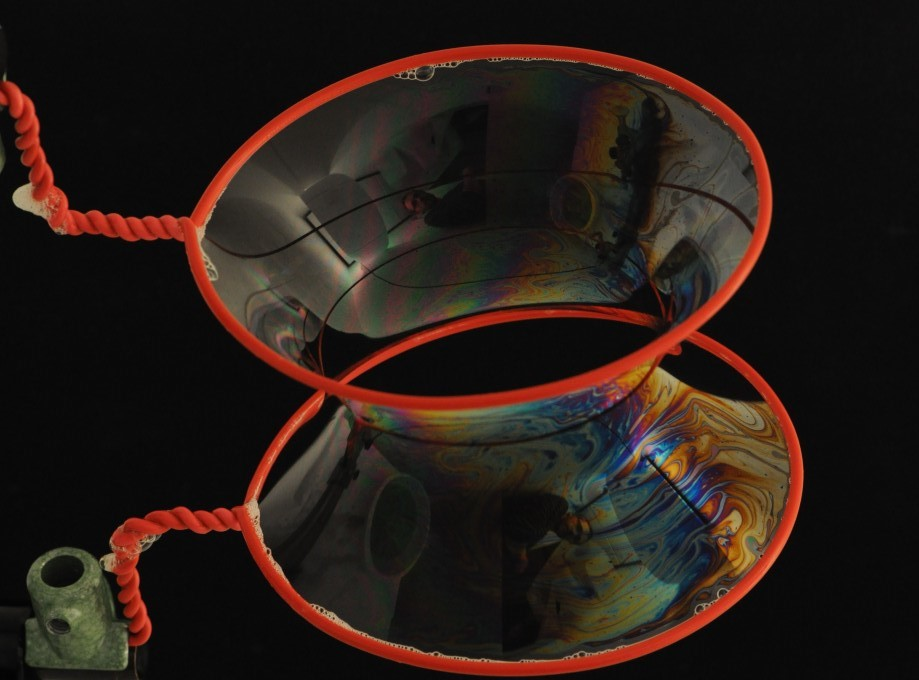
\includegraphics[width = 0.5 \linewidth]{Figures/01/soap_film.jpg}
    \caption{Pompa de jabón apoyada entre dos circunferencias paralelas y coaxiales.}
    \label{fig:pompa_fisica}
\end{figure}

La forma de equilibrio que adopta la superficie libre de este fluido es aquella que minimiza la energía total del sistema para el caso con las restricciones que se tengan. En esta energía, se han de tomar en consideración contribuciones como pueden ser:

\begin{itemize}
\item La energía debida a la \textbf{tensión superficial}, proporcional al área.
\item La \textbf{energía potencial}, debida a la gravedad y/o a la rotación como sólido rígido.
\end{itemize}

Este problema presenta una solución analítica para uno de los problemas más sencillos (sin considerar la gravedad ni otros parámetros): la catenoide. Para simplificar el trabajo se va a trabajar despreciando fuerzas másicas.

Suponiendo una superficie axilsimétrica, con un radio dado por
\(\rho=F(z)\), la energía superficial es proporcional (siendo la
constante de proporcionalidad la energía por unidad de área) a la
superficie, siendo esta proporcional (una vez adimensionalizada
adecuadamente) a:

\begin{equation} \label{eq:area}
    A = \int_0^1 F \sqrt{1 + \left( \frac{dF}{dz} \right)^2} dz
\end{equation}
donde se ha escogido la adimensionalización para que la distancia entre las superficies sea la unidad.

Imponiendo la minimización de la función \ref{eq:area} e imponiendo las condiciones en el contorno de $F(z = 0) = F(z = 1) = F_0$, se consigue resolver el problema.

Así, se va a estudiar la influencia de determinados parámetros del problema sobre la capacidad de encontrar una solución, así como sobre el propio algoritmo de optimización, comparando algoritmos tipo gradiente con otros heurísticos y evaluando los efectos de emplear cada uno de ellos. También, posteriormente, se estudiará la modificación del problema de optimización, provocando que la solución deje de ser simétrica o, por ejemplo, imponiendo restricciones sobre esta.

\section{Planteamiento del problema}

Para el desarrollo de los cálculos necesarios en este ejercicio, se ha desarrollado un Jupyter Notebook\cite{repositorio} que también se presenta y que detalla los aspectos de programación sobre la resolución del problema, limitándose este documento a las cuestiones relativas meramente a la optimización.

Por otro lado, si el lector estuviese interesado en comparar sus resultados con los aquí expuestos, ha de tener en cuenta que se han obtenido en un ordenador con procesador AMD Ryzen 5 3500U con una gráfica Radeon Vega Mobile Gfx 2.10 GHz, con 8,00 GB de RAM (6,94 GB usable) y sobre un sistema operativo de Windows 11 Home (Versión 23H2). Además, el código necesario se ha desarrollado íntegramente en un archivo Jupyter Notebook basado en Python y que se encuentra en el repositorio citado.


\subsection{Solución del problema físico}

Para el primer caso, existe solución analítica: la ya comentada catenoide (catenaria si se restringe el problema al plano), que sigue la siguiente ecuación:

\begin{equation} \label{eq:catenoide}
    F(z) = a \cosh \left( \frac{z + k}{a} \right)
\end{equation}
donde $a$ y $k$ son parámetros que dependen del problema que se esté considerando, por lo que habrá que resolverlos cada vez que se modifiquen las condiciones del problema. \footnote{$a = 0.848$ y $k = -0.500$ son los valores típicos para el problema más sencillo con $F(0) = F(1) = 1$.}

Esta es aplicable al problema sin restricciones de volumen, por lo que se va a emplear para comparar las soluciones numéricas obtenidas. 

\subsection{Parámetros de la minimización} \label{ap:params}

Para el primer estudio, se va a tratar aquel en el que los soportes son de igual radio: $F(z=0) = F(z=1) = F_0$. Además, se escoge arbitrariamente $F_0 = 1$. Más adelante, se estudiará cómo afecta la variación de este parámetro al cálculo de la solución.

En una primera aproximación, se estudiará para una partición equiespaciada y con un número $n$ arbitrario de puntos, en principio solo 20, ya que se verá que es más que suficiente, sin comprometer la potencia de cálculo necesaria para la solución.

El valor de los parámetros desde el que arranca la iteración se inicializa para el caso en el que $ F(z) = F_0 , \forall z \in [0, 1]$, es decir, en la posición en la que la superficie formaría un cilindro recto entre ambos soportes. 

Además del sentido físico que pueda tener considerar cómo evoluciona la pompa desde una posición próxima a la de equilibrio, interesa imponer estos valores de arranque por la proximidad de la solución a estos valores del radio, especialmente en las proximidades de los soportes. Posteriormente, se comentará el efecto de estas condiciones de arranque a la solución del problema.

\section{Problema sin restricciones, con soportes de igual tamaño}

En este apartado, se considera el problema más sencillo: la solución del problema sin ninguna condición adicional. A continuación, se van a comentar las consideraciones generales sobre los métodos de optimización, independientemente de si se trata de un algoritmo tipo gradiente o uno heurístico.

En primer lugar, pese a que inicialmente se considere un problema sin restricciones adicionales, no se puede ignorar el sentido físico del funcional que se quiere optimizar: el radio o distancia del eje a la superficie libre del fluido, magnitud que, por definición, es siempre no negativa. Así, se impone dicha frontera en el dominio ($F \geq 0$) para el cálculo de la solución del problema.

\subsection{Minimización con un método basado en gradiente}

En primer lugar, dentro de los métodos de tipo gradiente, se considerará el método de \textit{Sequential Least Squares Programming}\cite{ma2024improved}. Este algoritmo funciona aproximando la función objetivo y las restricciones mediante funciones cuadráticas en cada iteración y resolviendo estos subproblemas cuadráticos para actualizar la solución. Es eficiente y flexible, por lo que es el empleado para este trabajo.

A continuación, en la Figura \ref{fig:comp_grad_cat}, se muestra la comparación de la solución calculada con el método de gradiente y los parámetros enunciados y la solución analítica del problema. Estas apenas son distinguibles, ya que, con tan solo 20 puntos considerados, se obtiene un error cuadrático medio (SLE) \footnote{El error cuadrático medio se calcula a partir de la diferencia en cada valro de $z$ entre las posiciones calculadas con el algoritmo de optimización y el valor obtenido de la catenaria.} de 0.102\%, más que aceptable.

\begin{figure}[h]
    \centering
    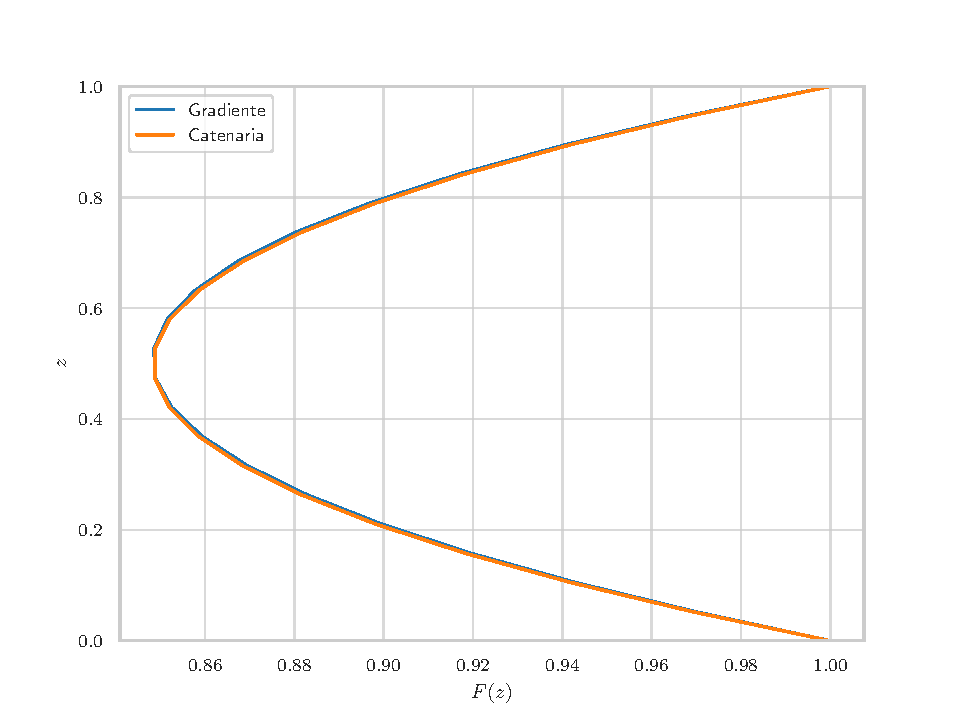
\includegraphics[width = 0.6 \linewidth]{Figures/01/comp_grad_cat.pdf}
    \caption{Comparación entre la solución analítica y la obtenida por el método del gradiente.}
    \label{fig:comp_grad_cat}
\end{figure}


\subsection{Minimización con un método heurístico}

Por contraposición al algoritmo tipo gradiente analizado anteriormente, a continuación se plantea la minimización del funcional a partir de un algoritmo heurístico, concretamente de \textit{Differential Evolution}\cite{DE_alg}.

El algoritmo de \textit{Differential Evolution} (DE) es una técnica de optimización global que pertenece a la familia de los algoritmos evolutivos. DE se utiliza principalmente para resolver problemas de optimización con variables continuas por sus ventajas frente a los algoritmos genéticos en este campo, como es el que se trata en el problema considerado.

Las soluciones se representan como vectores de números reales. Cada individuo en la población es un punto en el espacio de búsqueda multidimensional. La población inicial se genera de manera aleatoria dentro de los límites especificados para cada variable. Esto asegura una buena cobertura inicial del espacio de búsqueda.

A continuación, se detallan los operadores evolutivos que definen el DE:

\begin{itemize}
    \item \textbf{Mutación}: Genera un nuevo vector candidato sumando la diferencia ponderada entre dos vectores a un tercer vector. Este mecanismo introduce variabilidad basada en las diferencias entre individuos de la población.
    \begin{equation} \label{eq:mutacion}
        \mathbf{v}_i = \mathbf{x}_{r1} + F \cdot (\mathbf{x}_{r2} - \mathbf{x}_{r3})
    \end{equation}
    donde $\mathbf{x}_{r1}$, $\mathbf{x}_{r2}$ y $\mathbf{x}_{r3}$ son vectores aleatorios distintos seleccionados de la población, y $F$ es el factor de mutación que controla la amplitud de la variación diferencial.
    
    \item \textbf{Recombinación (Crossover)}: Combina el vector mutado con el vector actual del individuo para crear un nuevo vector de prueba. Esto se realiza seleccionando componentes del vector mutado y del vector actual basándose en una tasa de recombinación.
    
    \begin{equation}
        \mathbf{u}_{ij} = \begin{cases} 
        \mathbf{v}_{ij} & \text{si } \text{rand}(0,1) < CR \text{ o } j = \text{randint}(0,D-1) \\
        \mathbf{x}_{ij} & \text{de lo contrario}
        \end{cases}
    \end{equation}
    
    donde $\text{rand}(0,1)$ es un número aleatorio entre 0 y 1, y $\text{randint}(0,D-1)$ asegura que al menos un componente provenga del vector mutado.

    \item \textbf{Selección}: Compara el vector de prueba con el vector actual y selecciona el mejor (el que tenga la mejor aptitud) para la siguiente generación. Esto asegura que solo las soluciones más prometedoras sobrevivan.

    \begin{equation}
        \mathbf{x}_{i}^{(t+1)} = \begin{cases} 
        \mathbf{u}_i & \text{si } f(\mathbf{u}_i) \leq f(\mathbf{x}_i) \\
        \mathbf{x}_i & \text{de lo contrario}
        \end{cases}
    \end{equation}

    donde $f$ es la función objetivo a minimizar.
    
\end{itemize}


Así, se pueden extraer una serie de ventajas de emplear \textit{Differential Evolution}, entre las que destacan las siguientes:

\begin{itemize}
    \item \textbf{Simplicidad}: DE es fácil de implementar y requiere menos parámetros que muchos otros algoritmos evolutivos, como los algoritmos genéticos. Los principales parámetros son el tamaño de la población, el factor de mutación y la tasa de recombinación.

    \item \textbf{Eficiencia y convergencia}: DE es conocido por su eficiencia en la búsqueda global y su capacidad para converger a soluciones óptimas o cercanas al óptimo, incluso en espacios de búsqueda complejos con múltiples óptimos locales.

    \item \textbf{Robustez}: DE es robusto y eficaz en una amplia gama de problemas de optimización, incluidos aquellos con funciones objetivo no lineales y no convexas. La combinación de mutación y recombinación basada en diferencias permite una exploración efectiva del espacio de búsqueda.

    \item \textbf{Mantenimiento de la diversidad}: La mutación diferencial basada en las diferencias entre individuos ayuda a mantener la diversidad en la población, lo que es crucial para evitar el estancamiento en óptimos locales.
\end{itemize}

Precisamente, el DE resulta especialmente recomendado frente a los algoritmos genéticos para problemas donde las variables son continuas y el espacio de búsqueda es multidimensional.

Por tanto, en este trabajo se empleará DE por su implementación más sencilla, a través de la función \mintinline{python}{scipy.optimize.differential_evolution}\cite{2020SciPy-NMeth}, además de por los aspectos ya comentados. 

Esta función aproxima la solución por el método estudiado y, posteriormente, se acerca a la solución definitiva con unos pocos pasos de un algoritmo basado en gradiente. Así, realmente se está considerando un algoritmo híbrido (parte gradiente, parte heurístico), pero que permite extraer la solución calculada antes de detener la iteración con el DE, por lo que también se va a comentar.


\begin{figure}[h]
    \centering
    \begin{minipage}{0.45\textwidth}
        \centering
        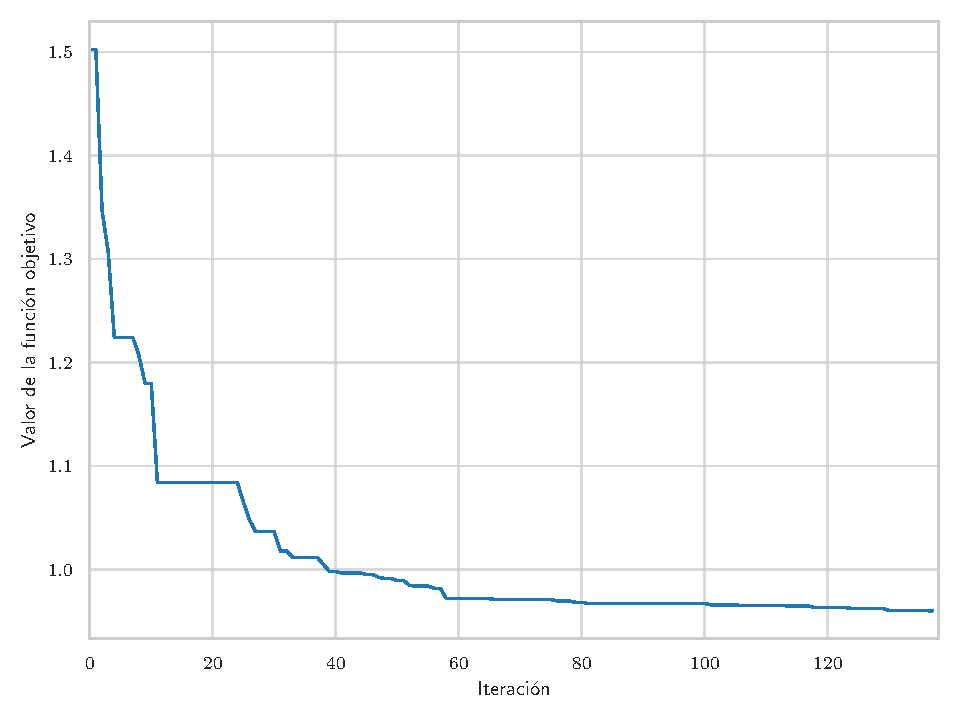
\includegraphics[width = \linewidth]{Figures/01/evol_de.pdf}
        \caption{Evolución de la optimización con \textit{Differential Evolution} en función de las iteraciones.}
        \label{fig:evol_de}
    \end{minipage}
    \hfill
    \begin{minipage}{0.45\textwidth}
        \centering
        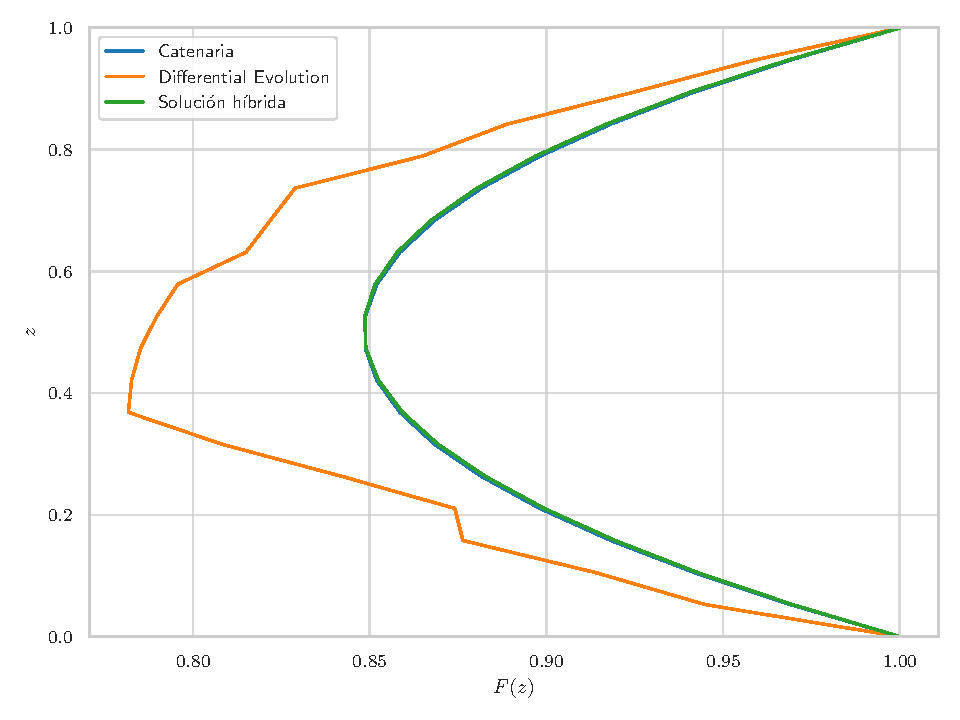
\includegraphics[width = \linewidth]{Figures/01/comp_de_cat.pdf}
        \caption{Comparación entre la solución analítica y la obtenida por \textit{Differential Evolution}.}
        \label{fig:comp_de_cat}
    \end{minipage}
\end{figure}

De la representación considerada en la Figura \ref{fig:comp_de_cat}, se puede visualizar claramente el efecto del algoritmo considerado. En primer lugar, se calcula una aproximación de la función con una tolerancia deseada, con el proceso representado en la Figura \ref{fig:evol_de}, tras la que se corta la iteración de este. De aquí, se toma el individuo con el mejor \textit{fitness} y se refina la solución con un algoritmo de tipo gradiente (concretamente L-BFGS-B\cite{L-BFGS-B}). 

Este procedimiento sigue siendo más costoso computacionalmente que emplear únicamente el algoritmo tipo gradiente, pero genera una solución de compromiso entre la precisión y rapidez de los algoritmos tipo gradiente y la flexibilidad de los algoritmos heurísticos, consiguiendo así un resultado más adecuado que si se emplease solo uno de los 2 tipos de algoritmos.


\subsection{Comparación entre el algoritmo tipo gradiente y el heurístico} \label{ap:comp_alg}

En primer lugar, se va a comparar el error entre la solución obtenida entre los métodos gradiente y heurístico, tomando también el valor para el que se detiene la evolución de la población del DE, a partir de los parámetros del problema definidos en \ref{ap:params}.

\begin{table}[h]
    \centering
    \caption{Error para los algoritmos considerados.}
    \begin{tabular}{c c}
        \hline
        \textbf{Algoritmo} & \textbf{SLE} [\%] \\ \hline \hline   
        SLSQP & 0.102 \\ \hline
        DE (detención de la evolución) & 4.909 \\ \hline
        DE afinado con L-BFGS-B & 0.096 \\ \hline
    \end{tabular}
    \label{tab:error_algs}
\end{table}

A raíz de los valores extraídos de la Tabla \ref{tab:error_algs}, se observa que ambos métodos obtienen una solución casi igual de precisa, si no más el DE, por lo que cabría pensar que este método es el mejor para calcular una solución al problema. Por otro lado, el valor que se observa antes de detener la evolución del DE es lo que se corresponde con la representación de la Figura \ref{fig:comp_de_cat}, un valor no demasiado cercano a la solución y que necesitaría de una cantidad ingente de generaciones para llegar a una solución con tolerancias admisibles.

Sin embargo, el error no es toda la información de la solución. Un punto muy importante a considerar es también el tiempo empleado en calcularla. En el caso de la solución calculada mediante SLSQP, ese tiempo empleado es de tan solo 0.17 s, mientras que, utilizando el \textit{Differential Evolution}, este tiempo asciende a unos nada despreciables 164.29 s.

Por tanto, queda considerar si una ligera mejora en la precisión y una mayor versatilidad compensan los desorbitados aumentos en la potencia de cálculo requerida. En este trabajo, ya que los algoritmos tipo gradiente no presentan una tendencia grande a atascarse en mínimos locales, se opta por realizar el análisis de la influencia de los parámetros solamente considerando estos, ya que, al afinar la solución del DE con un método basado en gradiente, se comportarán igual y permite analizar de una forma menos costosa el impacto de los parámetros del problema. 

\subsection{Influencia de los parámetros del problema} \label{ap:infl_params}

En este apartado, se va a estudiar el efecto de la variación de algunos parámetros del problema en la solución que se obtiene de este.

\subsubsection{Influencia del radio de los soportes, $F_0$}

En este apartado se va a considerar la variación del radio de los dos soportes, $F_0$, bajo la condición de que se mantenga igual en ambos, es decir, manteniendo $F(0) = F(1) = F_0$. Por otro lado, se congelan el resto de parámetros, manteniéndose igual que en el primer estudio.

Así, se recoge el valor del SLE para diferentes valores del radio de los soportes en la Tabla \ref{tab:error_radio}, así como su representación gráfica en la Figura \ref{fig:sol_radios}. 

\begin{table}[h]
    \centering
    \caption{Error para diferentes valores del radio.}
    \begin{tabular}{c c}
    \hline
        $\mathbf{F_0}$ & \textbf{SLE [\%]} \\ \hline \hline
        0.7 & 60.039 \\ \hline
        0.8 &  0.604 \\ \hline
        1   &  0.102 \\ \hline
        2   &  0.005 \\ \hline
        5   &  0.014 \\ \hline
    \end{tabular}
    \label{tab:error_radio}
\end{table}

\begin{figure}[h]
    \centering
    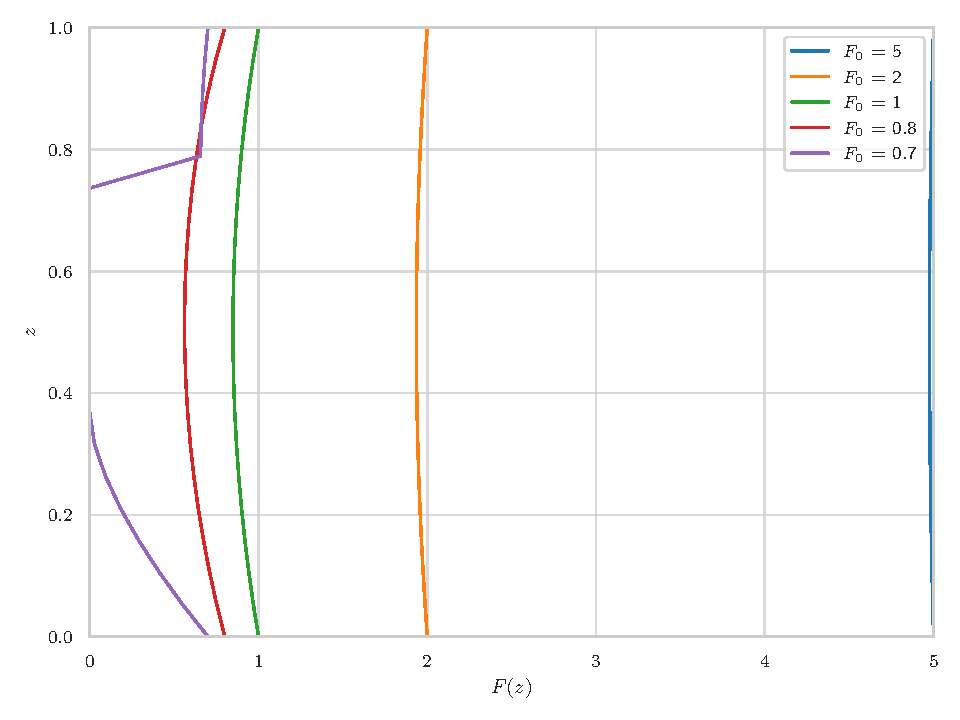
\includegraphics[width = 0.6 \linewidth]{Figures/01/sol_radios.pdf}
    \caption{Solución para distintos valores de $F_0$.}
    \label{fig:sol_radios}
\end{figure}

Como se observa en la Figura \ref{fig:sol_radios}, todos los casos en los que aumenta el valor de $F_0$ respecto de la unidad, presentan soluciones similares en cuanto a que se trata de una catenaria ajustada a esos puntos en el inicio y el final del intervalo.

Por otro lado, en los casos en los que $F_0$ decrece, se da un comportamiento anómalo. En valores mayores que $F_0 \approx 0.7$ no se produce ningún cambio de tendencia con respecto a lo observado anteriormente. Sin embargo, para condiciones de contorno con radios menores, la solución calculada presenta un comportamiento muy diferente, que puede dar lugar a pensar que es consecuencia de una falta de precisión del algoritmo de optimización, número de puntos insuficiente u otros problemas derivados de la aplicación numérica de los algoritmos de optimización. 

No obstante, modificando todos los valores que se mencionan no se consigue ninguna solución válida, lo que lleva a pensar que el alcance de los métodos empleados no permite calcular una solución en estos casos o bien que ni siquiera existe esa solución.


\subsubsection{Influencia del número de puntos de la discretización}\label{ap:infl_n}

A continuación, se tratará cómo afecta el número de puntos $n$ en los que se discretiza el intervalo $[0, 1]$, tomando para todos ellos el mismo esquema de partición equiespaciada y manteniendo el mismo valor de las condiciones de contorno y el resto de características del proceso.

\begin{table}[h]
    \centering
    \caption{Error y tiempo de ejecución para diferentes valores de $n$.}
    \begin{tabular}{c c c}
        \hline
        $\mathbf{n}$ & \textbf{SLE [\%]} & \textbf{Tiempo [s]} \\ \hline \hline
        5     & 0.377 &   0.017 \\ \hline
        10    & 0.194 &   0.039 \\ \hline
        20    & 0.102 &   0.148 \\ \hline
        50    & 0.065 &   1.048 \\ \hline
        100   & 0.034 &   6.838 \\ \hline
        200   & 0.131 &  27.507 \\ \hline
        400   & 2.873 & 106.424 \\ \hline
    \end{tabular}
    \label{tab:error_n}
\end{table}

\begin{figure}[h]
    \centering
    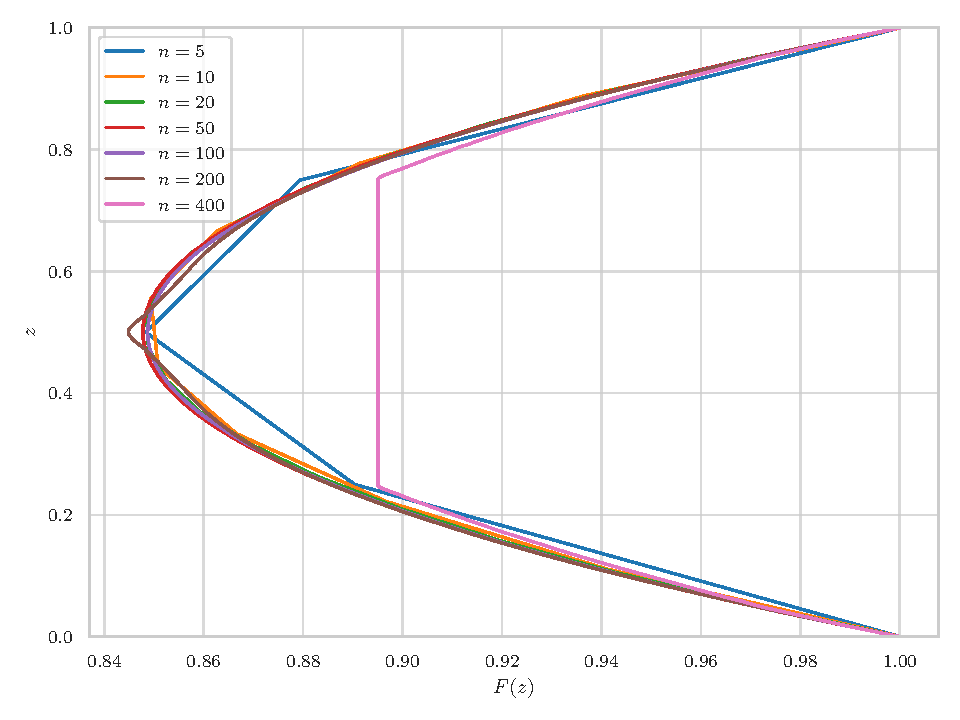
\includegraphics[width = 0.6 \linewidth]{Figures/01/sol_n.pdf}
    \caption{Solución para distintos valores de $n$.}
    \label{fig:sol_n}
\end{figure}

A raíz de los valores recogidos en la Tabla \ref{tab:error_n} y en la Figura \ref{fig:sol_n}, se pueden analizar los datos dividiéndolos en tres tendencias de comportamiento distintas y que se van a comentar a continuación por separado.

\begin{enumerate}
    \item \textbf{Pocos puntos} (5 ó 10 en la imagen): En estas curvas se aprecia el error del cálculo de la solución por el método empleado para el cálculo de la derivada. Este método presenta un error de truncamiento proporcional al tamaño del intervalo escogido entre puntos, y este es mayor cuanto menos puntos se escojan para aproximar la función.

    \item \textbf{Cantidad moderada de puntos} (entre 20 y 100 en la imagen): Estos esquemas son los que mejor se ajustan a la solución. Apenas se pueden apreciar cambios entre las curvas trazadas para dichos valores, por lo que se considera un valor de compromiso intermedio a fin de tener suficiente margen en la estabilidad de la solución.

    \item \textbf{Excesiva cantidad de puntos} (200, 400 o más): En este caso, los errores que se muestran son causa de la aproximación numérica de la derivada, pero esta vez asociada al error de redondeo. Este es el error asociado a la precisión finita del ordenador, proporcional a la constante de Lebesgue $\Lambda_n$, que, en el caso de una malla equiespaciada, es $\Lambda_n = \frac{2^n \sqrt{2}}{\pi n (n - 1)}$, donde $n$ es el número de puntos en los que se divide el intervalo. Es fácil observar que dicha constante puede alcanzar un valor muy alto, incluso para valores moderados de $n$. En el caso que se considera de 200 puntos, la cota inferior es $\Lambda_n \geq 1.8175e+55$, que,  aunque se multiplique por el valor de la precisión numérica de Python (del orden de $10^{-16}$), genera unas cotas de error para nada despreciables, pudiendo acarrear errores en la solución como los observados en la gráfica.
\end{enumerate}

Por tanto y por lo estudiado dentro de este apartado, se considera suficientemente preciso el número de puntos escogido ($n = 20$), consiguiendo un compromiso entre la precisión de la solución y la rapidez del cálculo de esta. 

Otra conclusión importante que se puede extraer de la Tabla \ref{tab:error_n} es que, al aumentar la resolución de la solución ($n$), el coste computacional aumenta a bastante mayor ritmo, por lo que es de vital importancia evaluar la cantidad de variables que son realmente necesarias en el problema para no comprometer la viabilidad computacional del cálculo de la solución, factor de vital importancia en la optimización de problemas en la industria.


\subsubsection{Influencia de la distribución de puntos} \label{ap:infl_distrib}

En este caso, se va a considerar el efecto de considerar diferentes distribuciones de puntos en las que dividir el intervalo del problema. 

Una vez más, se consideran el resto de parámetros idénticos al primer caso de estudio, salvo por el número de puntos $n$, que se va a modificar a fin de apreciar el comportamiento de distintas distribuciones de puntos en los casos más exigentes, es decir, en los casos extremos de $n$ muy grande o muy pequeño. El caso de $n$ intermedio se omite por presentar soluciones casi idénticas en todos los casos.

Así, en este apartado se estudiará la solución tomando la división del intervalo según los esquemas siguientes:

\begin{enumerate}
    \item Distribución de puntos \textbf{equiespaciada}.

    \item Distribución de puntos según un esquema de \textbf{ceros de Chebyshev}: 
    
    \begin{equation*}
        z_i = \cos{ \left( \frac{\frac{\pi}{2} + \pi i}{n + 1} \right) }, \quad i = 0, \dots , n
    \end{equation*}

    \item Distribución de puntos según un esquema de \textbf{extremos de Chebyshev}: 

    \begin{equation*}
        z_i =  \cos{ \left( \frac{\pi i}{n} \right) }, \quad i = 0, \dots , n
    \end{equation*}

    \item Distribución que \textbf{concentra puntos en el centro del intervalo}.

    Esta distribución se construye inicializando $n$ puntos equiespaciados en el intervalo $[-1, 1]$ y elevando el valor de cada uno de ellos al cubo, a fin de acercarlos a 0 (centro del intervalo). Después, se ajustan los extremos del intervalo que se considere ($[0, 1]$ en este trabajo). 
\end{enumerate}

\underline{\textbf{Caso de $n$ pequeño}}

En este caso, se considera el problema con $n = 10$, un número con el que se pueden obtener soluciones lo suficientemente precisas como para analizar si tiene efecto el esquema de la distribución de puntos en la solución.

\begin{table}[h]
    \centering
    \caption{Error para distintas distribuciones de puntos, con $n = 10$.}
    \begin{tabular}{c c}
        \hline
        \textbf{Distribución} & \textbf{SLS [\%]} \\ \hline \hline
        Equiespaciada              & 0.194 \\ \hline
        Ceros de Chebyshev         & 0.554 \\ \hline
        Extremos de Chebyshev      & 0.317 \\ \hline 
        Concentración en el centro & 1.229 \\ \hline
    \end{tabular}
    \label{tab:erorr_distrib_n10}
\end{table}

\begin{figure}[h]
    \centering
    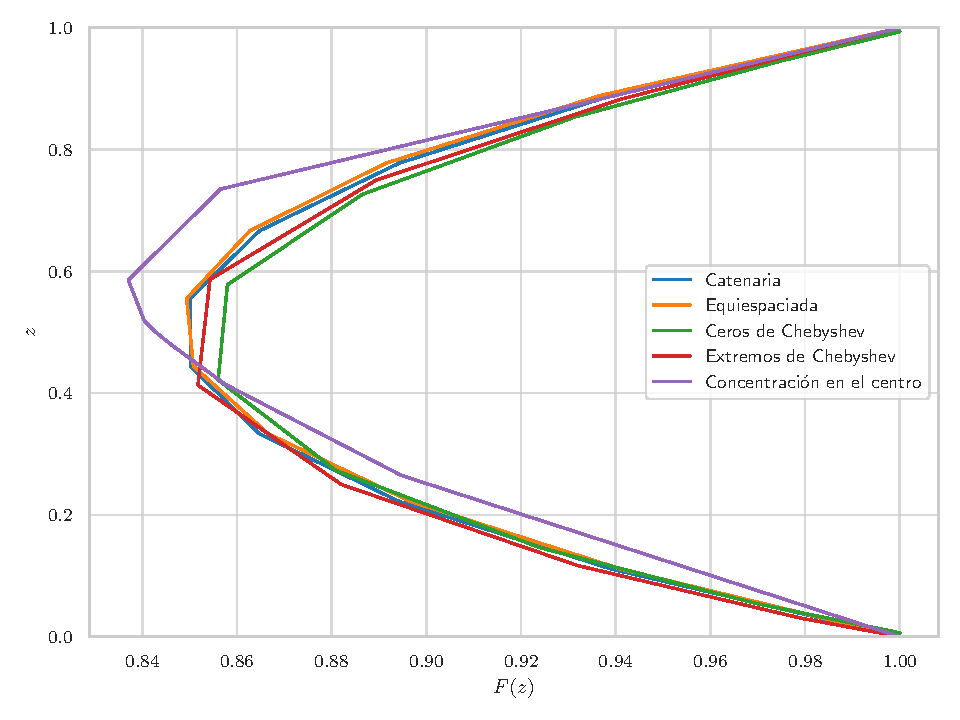
\includegraphics[width = 0.6 \linewidth]{Figures/01/sol_distrib_n10.pdf}
    \caption{Solución para distintas distribuciones de puntos, con $n = 10$.}
    \label{fig:sol_distrib_n10}
\end{figure}

En el caso expuesto, se aprecia en la Tabla \ref{tab:erorr_distrib_n10} y en la Figura \ref{fig:sol_distrib_n10} una solución que, aunque en los extremos del intervalo se parece mucho, no lo hace en la parte central. Esto es debido a que las distribuciones no equiespaciadas de tipo Chebyshev acumulan mayor cantidad de puntos en los extremos del intervalo mientras que, en el centro de este, el espaciado entre ellos es mayor, provocando así que la aproximación de la solución sea más imprecisa, por el mismo motivo que se comentó sobre la influencia del número de puntos anteriormente. 

Por otro lado, se observa que la que peor comportamiento presenta es la que concentra puntos en el centro, por lo que parece que no resulta una distribución adecuada para este problema.


\underline{\textbf{Caso de $n$ grande}}

Por otro lado, se toma el problema discretizado en 200 puntos, para analizar el otro extremo del caso en el que se varía el esquema de partición del intervalo.

\begin{table}[h]
    \centering
    \caption{Error para distintas distribuciones de puntos, con $n = 200$.}
    \begin{tabular}{c c}
        \hline
        \textbf{Distribución} & \textbf{SLS [\%]} \\ \hline \hline
        Equiespaciada              & 1.808 \\ \hline
        Ceros de Chebyshev         & 1.202 \\ \hline
        Extremos de Chebyshev      & 0.669 \\ \hline 
        Concentración en el centro & 15.470 \\ \hline
    \end{tabular}
    \label{tab:erorr_distrib_n200}
\end{table}

\begin{figure}[h]
    \centering
    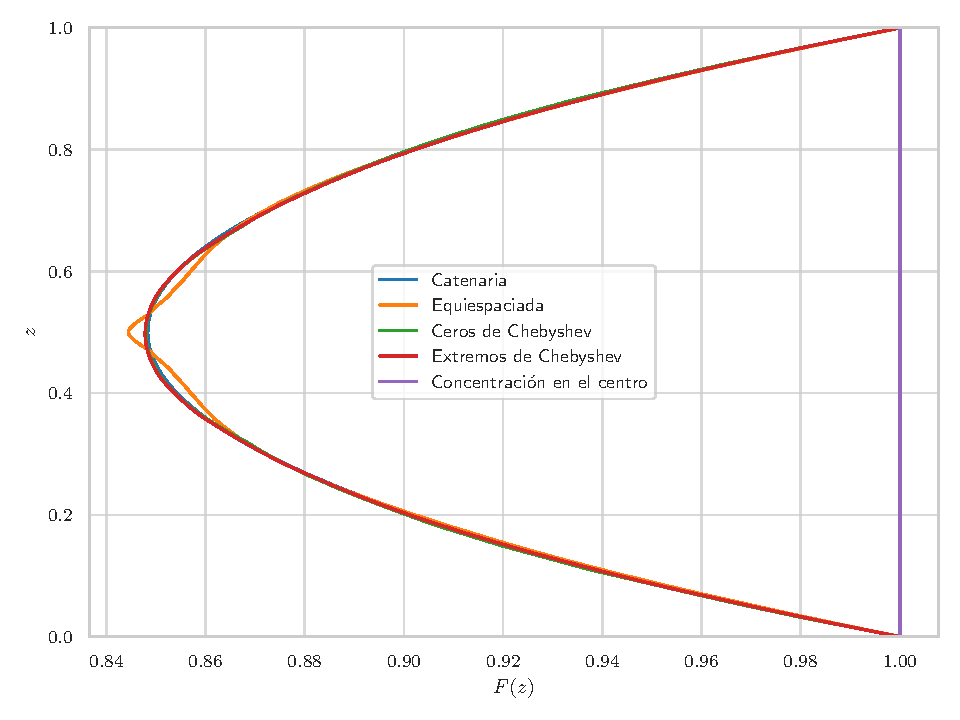
\includegraphics[width = 0.6 \linewidth]{Figures/01/sol_distrib_n200.pdf}
    \caption{Solución para distintas distribuciones de puntos, con $n = 200$.}
    \label{fig:sol_distrib_n200}
\end{figure}

De forma opuesta que en el caso anterior, como se aprecia en la Tabla \ref{tab:erorr_distrib_n200} y en la Figura \ref{fig:sol_distrib_n200}, ahora las distribuciones que mejor se comportan (dentro del mal comportamiento general) son las no equiespaciadas de tipo Chebyshev. En este caso se debe a que, como se comentó en el apartado \ref{ap:infl_n}, las distribuciones equiespaciadas presentan un error de redondeo que se dispara al aumentar el número de puntos, que es lo que ocurre en este caso. 

Al contrario, las distribuciones no equiespaciadas de tipo Chebyshev acumulan más puntos en los extremos, consiguiendo adaptarse así mejor, y manteniendo una densidad de puntos moderada en los puntos centrales, reduciendo así el error de redondeo. 

Por último, se aprecia un comportamiento paupérrimo para la distribución que concentra puntos en el centro del intervalo, por lo que se descarta su aplicación en ninguno de los casos.

\subsubsection{Influencia del esquema de cálculo de derivadas}

En este caso, se pasará a estudiar la influencia del esquema de derivación en la solución obtenida del problema. Los esquemas de diferencias finitas que se consideran para el cálculo son algunos de los más sencillos, estudiados en la asignatura.

Para ello, en primer lugar, se especifican los esquemas que se emplearán:

\begin{enumerate}
    \item \textbf{Diferencias finitas progresivas}: 
    
    \begin{equation}
        \frac{d F}{d z} \cong \frac{F(z + \delta_z) - F(z)}{\delta_z}
    \end{equation}

    \item \textbf{Diferencias finitas regresivas}: 
    
    \begin{equation}
        \frac{d F}{d z} \cong \frac{F(z) - F(z - \delta_z)}{\delta_z}
    \end{equation}

    \item \textbf{Diferencias finitas centradas}: 
    
    \begin{equation}
        \frac{d F}{d z} \cong \frac{F(z + \delta_z) - F(z - \delta_z)}{2 \delta_z}
    \end{equation}
\end{enumerate}

A continuación, se va a observar el efecto del esquema de cálculo de la derivada en función del número de puntos escogidos, en todos los casos bajo el mismo esquema equiespaciado de partición del intervalo. 

\begin{table}[h]
    \centering
    \caption{Error para distintos esquemas de diferencias finitas y valores de $n$.}
    \begin{tabular}{|c|c|c|c|c|}
        \hline
         & \multicolumn{4}{|c|}{\textbf{SLE [\%]}} \\ \hline 
        \diagbox{\textbf{Esquema}}{\textbf{n}} & 10 & 100 & 200 & 400 \\ \hline
        Adelantado & 0.560 & 0.305 & 1.664 & 118.665 \\ \hline
        Retrasado  & 0.560 & 0.688 & 1.808 & 118.662 \\ \hline
        Centrado   & 6.140 & 2.592 & 2.068 &  32.935 \\ \hline
    \end{tabular}
    \label{tab:error_diff}
\end{table}

\begin{figure}[h]
    \centering
    \begin{subfigure}[b]{0.45\textwidth}
        \centering
        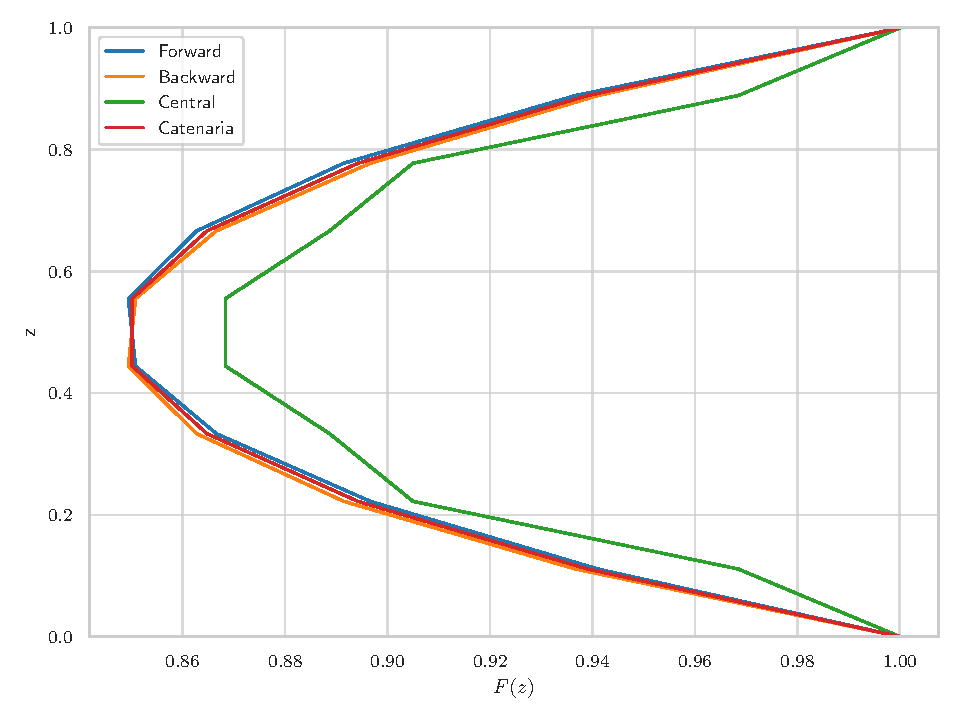
\includegraphics[width=\textwidth]{Figures/01/sol_deriv_n10.pdf}
        \caption{$n = 10$}
        \label{fig:diff_n10}
    \end{subfigure}
    \hfill
    \begin{subfigure}[b]{0.45\textwidth}
        \centering
        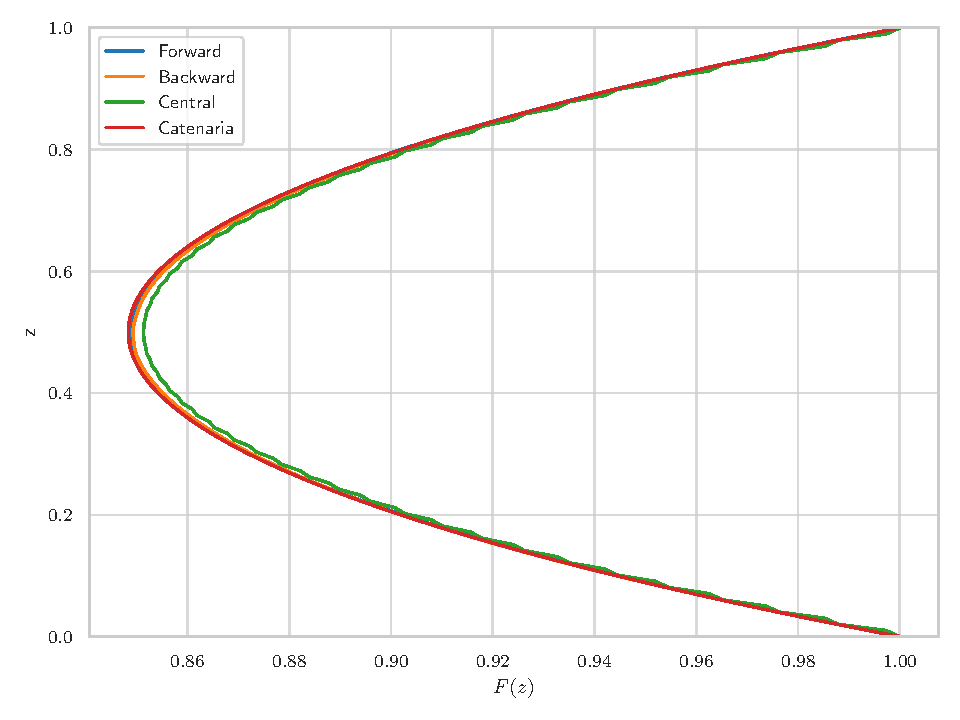
\includegraphics[width=\textwidth]{Figures/01/sol_deriv_n100.pdf}
        \caption{$n = 100$}
        \label{fig:diff_n100}
    \end{subfigure}

    \vspace{1em} % Espacio vertical entre las filas

    \begin{subfigure}[b]{0.45\textwidth}
        \centering
        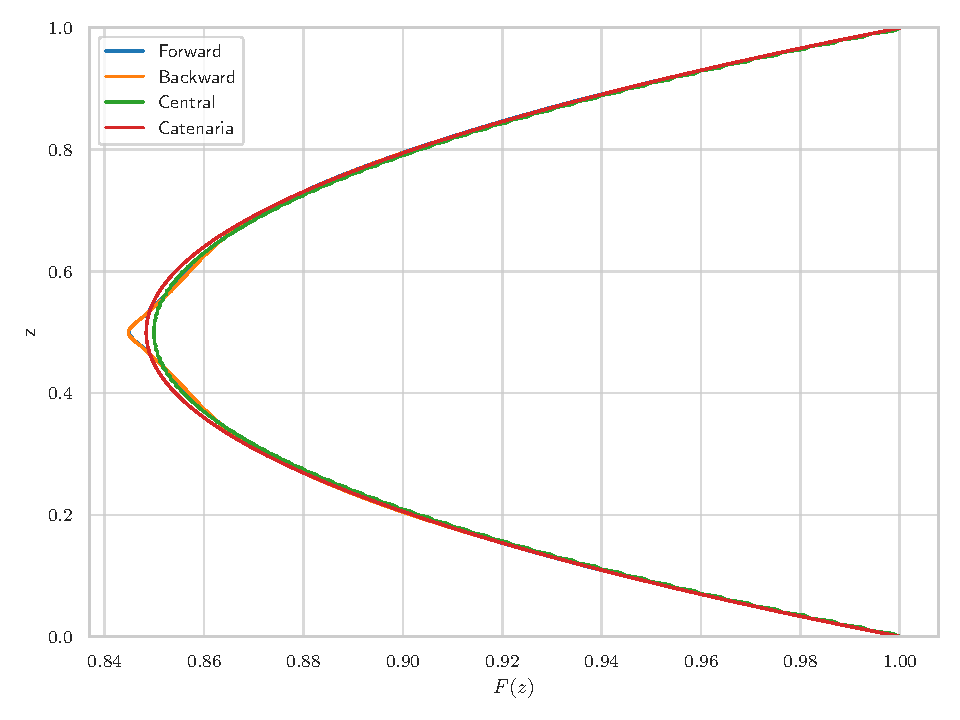
\includegraphics[width=\textwidth]{Figures/01/sol_deriv_n200.pdf}
        \caption{$n = 200$}
        \label{fig:diff_n200}
    \end{subfigure}
    \hfill
    \begin{subfigure}[b]{0.45\textwidth}
        \centering
        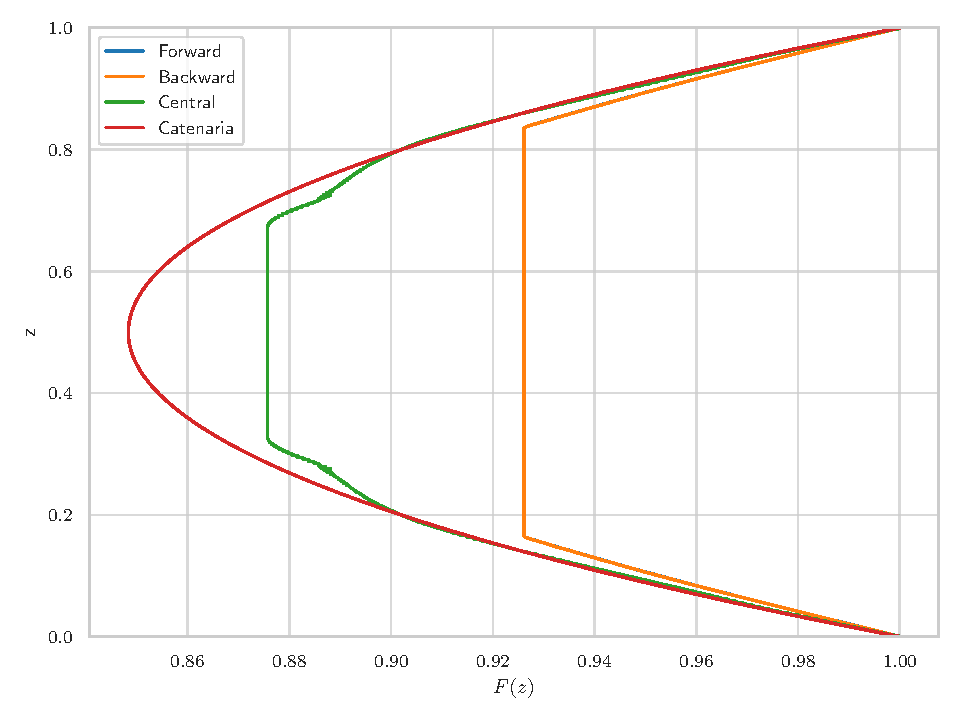
\includegraphics[width=\textwidth]{Figures/01/sol_deriv_n600.pdf}
        \caption{$n = 600$}
        \label{fig:diff_n600}
    \end{subfigure}
    \caption{Solución para distintos esquemas de diferencias finitas y valores de $n$.}
    \label{fig:sol_diff}
\end{figure}

Antes de nada, cabe reseñar la proximidad de la solución de las diferencias finitas adelantadas y las retrasadas, tendencia que se va a mantener para todos los casos recogidos en la Tabla \ref{tab:error_diff} y en la Figura \ref{fig:sol_diff}, por lo que, cuando se hable de diferencias finitas descentradas en lo que sigue, se hará referencia a ambas para evitar repeticiones innecesarias.

En el caso con pocos puntos, recogido en la Figura \ref{fig:diff_n10}, se puede apreciar como las diferencias finitas descentradas generan un mejor resultado en la aproximación de la solución. Esto es debido a que el paso en la fórmula de las diferencias finitas centradas es el doble que en las otras, por lo que se produce un cambio más pronunciado en las propiedades en ese espaciado que en las descentradas, acarreando así mayor error en la aproximación de la función. 

En el caso de escoger una cantidad moderada de puntos, se observa en la Figura \ref{fig:diff_n100} un comportamiento similar al estudiado en el caso anterior. Sin embargo, en este caso, las diferencias finitas centradas se acercan aún más al resultado de las fórmulas descentradas. Esto se produce porque, al aumentar tanto el espaciado, aunque el paso sea mayor que en el caso de las fórmulas descentradas, presenta una aproximación cada vez más aceptable de la solución.   

Al contrario que en los casos estudiados para menor cantidad de puntos, al aumentar lo suficiente $n$ se produce un cambio de tendencia, como es visible en las Figuras \ref{fig:diff_n200} y \ref{fig:diff_n600}. 

En el caso de la Figura \ref{fig:diff_n200}, ningún esquema proporciona un gran resultado, aunque el que emplea un cálculo de la derivada siguiendo un esquema de diferencias finitas centradas mantiene un nivel de fidelidad con la solución comparable con las descentradas. Precisamente, el cambio respecto a lo considerado anteriormente se debe al mismo motivo por el que antes no se conseguía una aproximación tan buena: que el paso sea el doble que en las diferencias finitas descentradas. 

Al crecer tanto el error de redondeo (según la constante de Lebesge, $\Lambda$), las diferencias finitas descentradas para una malla equiespaciada dejan de ser una opción viable en cuanto aumenta el número de puntos por encima de un umbral relativamente bajo. Es así que, para mallas con muchos puntos, se recomienda cambiar el esquema a uno de derivadas finitas centradas.

Aunque en el caso de la Figura \ref{fig:diff_n600} se consideren “tan solo” 600 puntos, es un buen indicador del efecto que tiene aumentar la cantidad de puntos por encima de un límite admisible, o lo que es lo mismo, en el límite de $n \to \infty$. 

Aquí, se observa que sendos esquemas descentrados y centrados sufren errores, una vez más debidos al error de redondeo, a su vez proporcional a la constante de Lebesgue. En este caso, tanto el esquema centrado de cálculo de diferencias finitas como, evidentemente, los esquemas descentrados, presentan amplitudes de los intervalos tan pequeñas entre los puntos que se evalúa la función que el error numérico al dividir por valores tan pequeños se dispara, provocando estas soluciones que para nada se parecen a la solución real del problema.

\subsubsection{Influencia del valor de arranque de la iteración}

Otro parámetro que puede influir en las características de la solución obtenida es el valor que se escoja de arranque en la iteración, lo que equivale al punto escogido desde el que arrancar el método de basado en gradiente que se escoja. 

En principio, se ha escogido para este valor un caso de $F(z) = F_0 , \forall z \in [0, 1]$, pero a continuación se propone inicializar en distintos valores, que se detallan a continuación. En todos estos se considera $F_0 = 1$, por lo que se omite en las expresiones.

Casos del valor de arranque considerados:

\begin{enumerate}
    \item $F(z) = 1 , \forall z \in [0, 1]$
    
    \item $F(z) = 0 , \forall z \in [0, 1]$

    \item $F(z) \leq 0.6 , \forall z \in [0, 1]$

    \item $0.6 < F(z) < 2 , \forall z \in [0, 1]$

    \item $F(z) \gg 2 , \forall z \in [0, 1]$
    
    \item $F(z) \sim \text{U}(0.6, 2)$
\end{enumerate}

Como en este caso se evalúa si se alcanza o no la solución, no se va a representar la solución \footnote{Resultaría demasiado engorroso representar las soluciones de una en una para comparar si llegan o no a una solución válida, por lo que no se incluye en este documento, pero sí en el código adjunto.}, sino que se va a atender al mensaje de parada del algoritmo de optimización \footnote{Si alcanza con éxito el mínimo o no, atendiendo al mensaje que arroja la función de si se alcanza un punto con el gradiente nulo o si se alcanza el valor máximo de iteraciones.} y al valor del error de la solución, recogidos en la Tabla \ref{tab:variar_F}.

\begin{table}[h]
    \centering
    \caption{Resultados de la optimización con cada uno de los casos de valores de arranque.} 
    \begin{tabular}{|c|c|c|}
        \hline
        \textbf{Caso} & \textbf{¿Éxito?} & \textbf{SLE [\%]} \\ \hline \hline
        1 & Sí &  0.102 \\ \hline
        2 & Sí & 80.909 \\ \hline
        3 & Sí & 80.899 \\ \hline
        4 & Sí &  0.093 \\ \hline
        5 & Sí & 80.902 \\ \hline
        6 & Sí & 80.902 \\ \hline
    \end{tabular}
    \label{tab:variar_F}
\end{table}

Como se ha comprobado en apartados anteriores, al alcanzar un valor del error de aproximadamente un $0.1 \% $ se considera que la función ha llegado al mínimo que permiten las condiciones del problema. Por tanto, para comparar si la solución a la que ha convergido cada método es la correcta, se procederá a comparar dichos valores.

Por tanto, de los valores de la Tabla \ref{tab:variar_F}, se observa que solo alcanzan un resultado válido los casos 1 y 4, pese a que el algoritmo indica que se ha llegado a un mínimo. Además del valor del error que se muestra en la Tabla \ref{tab:variar_F}, otra pista que puede denotar que realmente no estamos ante una solución válida es la forma que tiene esta, recogida en la Figura \ref{fig:sol_cambioF0}, que, aunque solo esté representada la solución con el caso 3, refleja también el comportamiento de los casos 2, 5, y 6.

\begin{figure}[h]
    \centering
    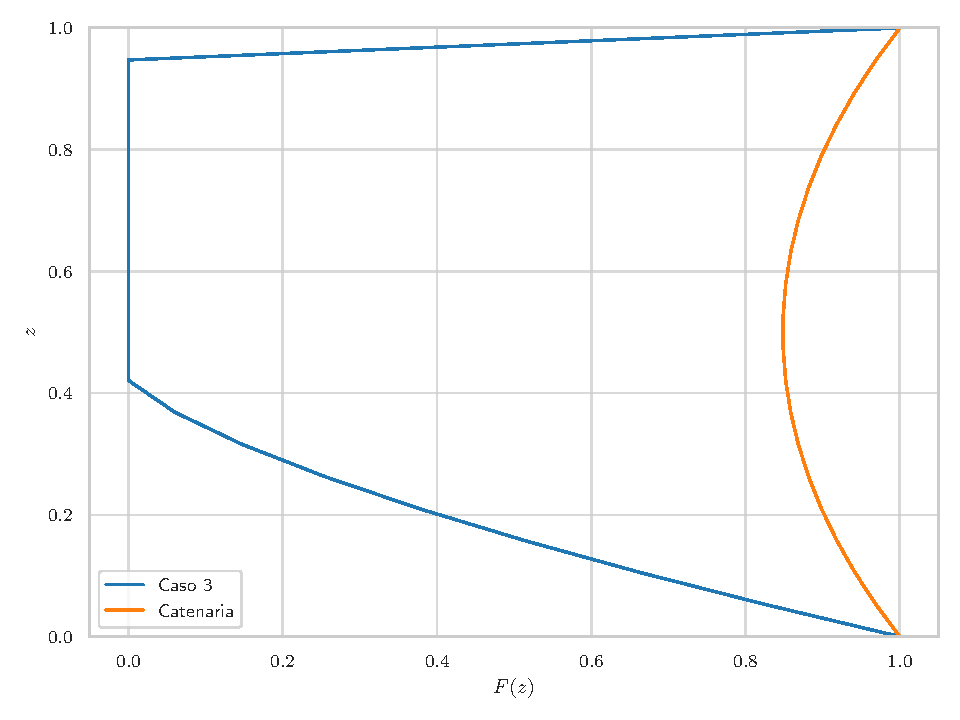
\includegraphics[width = 0.6 \linewidth]{Figures/01/sol_cambioF0.pdf}
    \caption{Solución para el error típico de 81 \%.}
    \label{fig:sol_cambioF0}
\end{figure}

De este apartado se extraen una serie de conclusiones. La primera de ellas es que no es necesario que el algoritmo arranque exactamente en el valor de $F_0$, ya que eso provocaría muy poca robustez en la resolución del problema. Existe un intervalo que llamaremos “zona válida de arranque” en la que los valores de la función pueden inicializarse y el algoritmo conseguirá converger para llegar a la solución adecuada. 

En segundo lugar, como se comprueba en los casos 2 y 3, se encuentra que para valores iniciales de la iteración demasiado cercanos al origen, el algoritmo no es capaz de converger a la solución correcta. Por otro lado, al igual que en los puntos por debajo de la cota inferior de la zona válida de arranque, los que se sitúan por encima llegan a una solución inadecuada, y esto se mantiene para todos los valores mayores que 2, según el análisis que se ha llevado a cabo.

Del caso 6 se concluye que, arrancando con valores altamente irregulares, pese a que estos se encuentren todos dentro de la zona válida de arranque, no se alcanza una solución válida. Aunque se ha comprobado que existe la posibilidad de que el algoritmo converja a la solución correcta, lo cierto es que esto apenas sucede unas pocas veces y es imposible predecir en qué casos lo hará, por lo que no se considera un método robusto en el que se sepa que se va a alcanzar una solución óptima.

Así, se concluye en este apartado es que el valor de arranque resulta un parámetro crucial en la capacidad de llegar a una solución óptima. Sobre el valor que se podría escoger a ciegas, conviene guiarse por el sentido físico del problema, así como por las condiciones de contorno, sabiendo que los valores próximos a los extremos del intervalo han de ser similares a los valores de la condición de contorno.


\subsection{Consideraciones particulares}

Además de los parámetros evidentes que se pueden alterar y se han comentado en el Apartado \ref{ap:infl_params}, se plantean a continuación unas condiciones muy particulares para las que se quiere estudiar el comportamiento de la solución.

\subsubsection{Arranque de la iteración del algoritmo gradiente en la solución}

Para evaluar la precisión del modelo con el que se trabaja, además de a fin de evaluar el comportamiento que tiene el método gradiente, se plantea arrancar la iteración de este método con la solución analítica obtenida a partir de la catenaria, para ver con qué precisión se calcula dicha solución. 

Si el modelo representase la realidad sin ninguna imprecisión en el cálculo ni en la construcción del modelo, el algoritmo debería detenerse en el primer paso de la iteración y mantenerse en el mismo punto, ya que este es el mínimo del modelo real. Para evaluar este comportamiento, se va a reducir progresivamente la tolerancia de convergencia del modelo, lo que debería mejorar la precisión de este. Dichos datos se recogen en la Tabla \ref{tab:tol}.

\begin{table}[h]
    \centering
    \begin{tabular}{|c|c|c|c|}
        \hline
        \textbf{Tolerancia} & \textbf{Iteraciones} & \textbf{Norma del gradiente} & \textbf{SLE [\%]} \\ \hline \hline
        1e-05 &  1 & 6.526e-02 & 0.041 \\ \hline
        1e-07 & 11 & 2.729e-02 & 0.085 \\ \hline
        1e-10 & 22 & 1.453e-05 & 0.095 \\ \hline
        1e-13 & 24 & 2.779e-06 & 0.095 \\ \hline
        1e-16 & 69 & 7.489e-07 & 0.095 \\ \hline
    \end{tabular}
    \caption{Convergencia en función de la tolerancia.}
    \label{tab:tol}
\end{table}

A partir de estos datos, se observa que solo el valor con mayor tolerancia para en la primera iteración. El resto, que precisan de más iteraciones para converger, se comportan así porque el modelo del problema planteado no recoge con toda la precisión que requeriría para igualar la solución analítica.

Por otro lado, se observa que, al reducir el valor de la tolerancia, el algoritmo se comporta como cabría esperar: aumenta el número de iteraciones hasta llegar al punto mínimo del modelo, se reduce el valor del gradiente (que es lo que marca la parada) y el error aumenta (ya que se aleja del punto de error nulo, donde se arranca la iteración).


\subsubsection{Arranque de la iteración del algoritmo heurístico en la solución}

Otra pregunta que se puede plantear es lo mismo, pero en el caso del algoritmo de \textit{Differential Evolution} considerado. En este caso, sin importar la tolerancia que se imponga, siempre se detiene en la primera iteración, consiguiendo la solución igual a la extraída de la catenaria.

Sin embargo, este comportamiento puede llegar a engaños, ya que, según se puede observar en la Ecuación \ref{eq:mutacion}, la estrategia de mutación del algoritmo DE no introduce la mutación aleatoria que sí introduciría, por ejemplo, un algoritmo genético. Por eso mismo, es imprescindible arrancar la iteración con una población lo suficientemente diversa como para que las generaciones no se estanquen demasiado pronto. 


\subsection{Solución obtenida de la ecuación de Euler}

Este problema, además de calcularse por minimización del área, admite otra resolución mediante la ecuación de Euler. Dicha ecuación, también conocida como la ecuación de Euler-Lagrange, afirma que el funcional genérico

\begin{equation}
    J[y(x)] = \int_a^b \mathcal{L}(x, y, y')
\end{equation}
debe verificar la siguiente ecuación diferencial de segundo orden \cite{gelfand2000calculus}: 

\begin{equation}
    \frac{\partial\mathcal{L}}{\partial y} - \frac{d}{dx}\frac{\partial\mathcal{L}}{\partial y'} = 0
\end{equation}

Esta ecuación diferencial será, en general, no lineal, y deberá resolverse con dos condiciones iniciales o de contorno. En el problema a estudiar, el funcional es el área, definida en la Ecuación \ref{eq:area}, y las dos condiciones de contorno a imponer son $F(z = 0) = F(z = 1) = F_0$. Realizando ciertos cálculos simples, se obtiene la siguiente ecuación a resolver: 

\begin{equation}
    F(z) F''(z) - (F'(z))^2 = 1
\end{equation}

Esta ecuación tiene la solución analítica expuesta en la Ecuación \ref{eq:catenoide}. La primera constante de integración tomará el valor $k = -0.5$, mientras que la segunda se obtendrá de resolver la siguiente ecuación no lineal: 

 \begin{equation}
     a \cosh \left( \frac{1}{2a} \right) = 1
 \end{equation}
 cuya solución aproximada es, como se afirmaba anteriormente, $a = 0.848$. 

Si se desea resolver dicha ecuación numéricamente, lo más adecuado es utilizar el método del disparo (dado que se trata de una EDO no lineal con valores en la frontera). 

\begin{figure}[h]
    \centering
    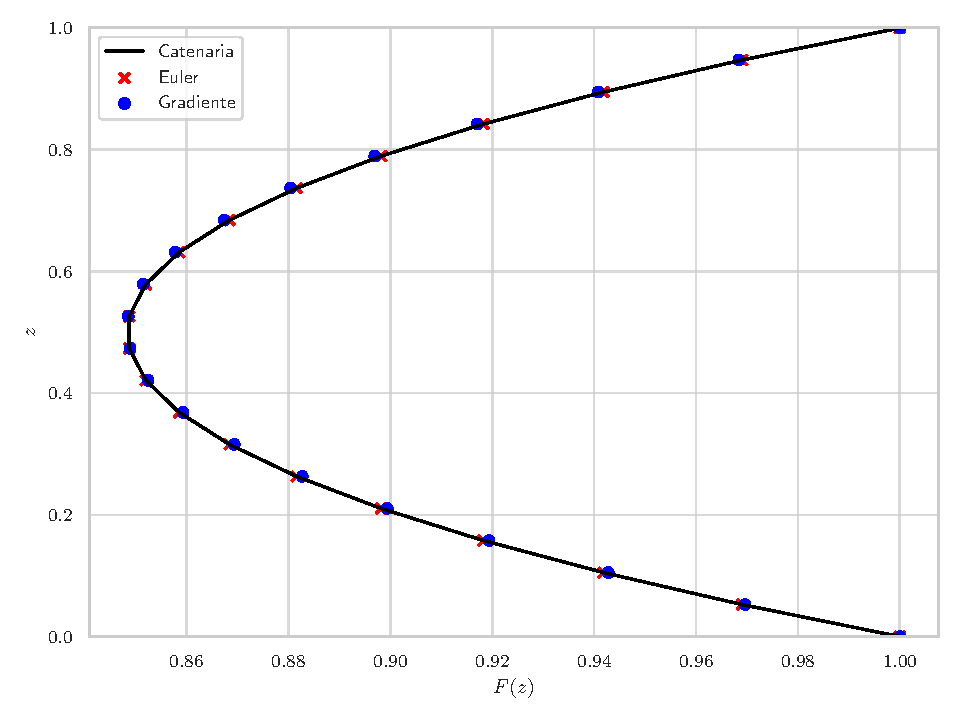
\includegraphics[width = 0.6 \linewidth]{Figures/01/sol_euler.pdf}
    \caption{Comparativa de las soluciones por distintos métodos.}
    \label{fig:sol_euler}
\end{figure}

Así, de la solución representada en la Figura \ref{fig:sol_euler}, se comprueba que la solución de la ecuación de Euler se ajusta a la catenaria y, a su vez, sirve para corroborar una vez más que la optimización llevada a cabo por el método de gradiente es fiel a la realidad.

\section{Problema con restricciones de volumen, con soportes de igual tamaño}

En el análisis de este apartado se fija como restricción a la solución el volumen encerrado por la superficie y los planos que contienen a las 2 circunferencias para ver su efecto sobre la solución del problema. Este volumen se calcula con la siguiente expresión:

\begin{equation}
    V = \int_0^1 F^2 dz
\end{equation}

En primer lugar, se calcula el valor del volumen de la solución sin restricciones, que resulta ser de 0.8095. Este valor se toma de referencia según se quiera reducir o aumentar y ver la influencia que tiene sobre la solución. 

Cabe mencionar que, salvando particularidades como pueden ser el caso en que la restricción coincida con el volumen del problema sin restricciones o un caso en el que la solución represente un cilindro recto, no se puede analizar el error de la solución como se ha realizado en el anterior apartado, por lo que, para observar si la solución cumple las condiciones se atenderá únicamente a la representación gráfica de esta.

\subsection{Minimización con un método basado en gradiente} \label{ap:cons_grad}

Como en el anterior apartado, se va a comenzar el análisis por el caso en que se calcula la solución mediante un método gradiente. La estrategia que se va a seguir es calcular la solución, alterando el valor del volumen tanto por encima como por debajo de la obtenida sin restricciones y observar en qué valores deja de tener sentido esta, encontrando el límite del volumen encerrado para el problema. \footnote{Se mantienen el resto de valores considerados en el apartado \ref{ap:params}.}

\begin{figure}[h]
    \centering
    \begin{subfigure}[b]{0.45\textwidth}
        \centering
        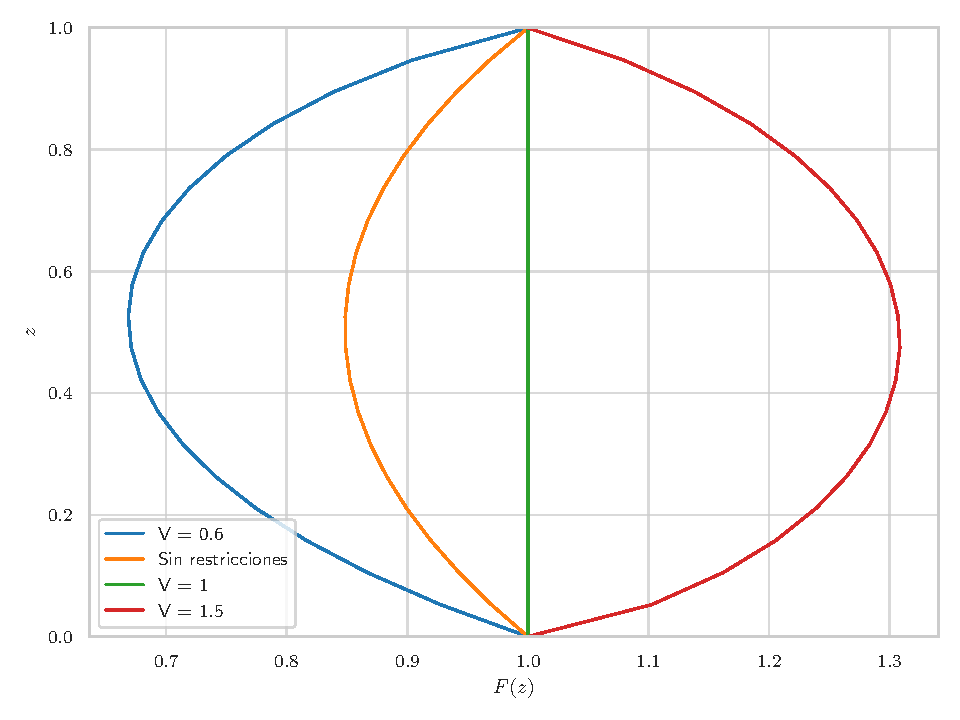
\includegraphics[width=\textwidth]{Figures/01/vol_inic.pdf}
        \caption{Soluciones válidas.}
        \label{fig:vol_inic}
    \end{subfigure}
    \hfill
    \begin{subfigure}[b]{0.45\textwidth}
        \centering
        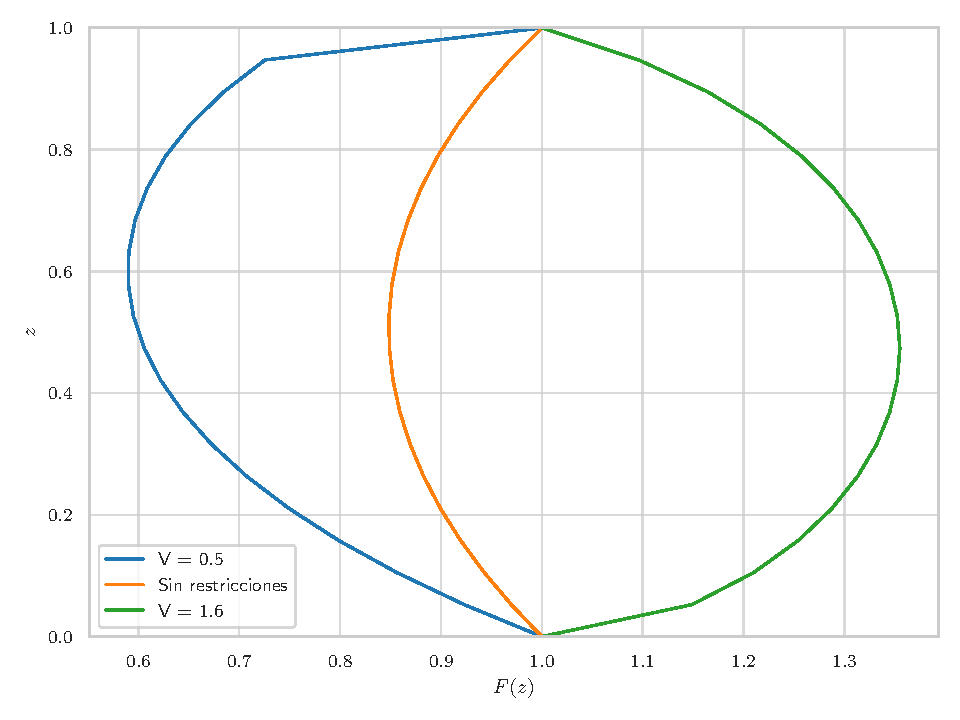
\includegraphics[width=\textwidth]{Figures/01/vol_no_sol.pdf}
        \caption{Soluciones no válidas.}
        \label{fig:vol_no_sol}
    \end{subfigure}
    \caption{Solución para distintos valores de la restricción de volumen, con método gradiente.}
    \label{fig:vol_variacion}
\end{figure}

Así, en la Figura \ref{fig:vol_variacion} se representan las soluciones que sí se consideran aceptables (\ref{fig:vol_inic}) y las que no (\ref{fig:vol_no_sol}). Como cabía esperar, la forma de la solución se modifica al aumentar el valor de la restricción de volumen. Es importante recalcar que esta restricción no puede tomar cualquier valor, ya que, si difiere en gran medida del volumen obtenido sin restricciones, la solución puede resultar inexistente o inestable. 

De las soluciones que se recogen en la Figura \ref{fig:vol_no_sol} se aprecia que, como poco, no tienen sentido físico. Por tanto, en primera aproximación, se obtiene una cota superior para la restricción de aproximadamente $1.5$ y una inferior de aproximadamente $0.6$. Cabe pensar que, para los casos más sensibles (los más cercanos a las soluciones válidas), pueda existir solución, solo que el método no tiene la precisión adecuada para calcularlo. Así, se plantea evaluar el efecto de aumentar el número de puntos, a fin de tener una representación más precisa.% por lo que a continuación se estudiarán los parámetros que pudieran tener influencia para determinar el mínimo y máximo valor de la restricción con la que se obtiene una restricción válida. 



\subsection{Minimización con método heurístico}

Por otro lado, se quiere comprobar si empleando un método heurístico pudiese mejorar la solución en el caso de estar considerando una restricción.

Cabe destacar que imponer una restricción en un método heurístico resulta bastante más complejo que en un gradiente, por el carácter de aleatoriedad que incorpora. Aunque en el caso de este trabajo, la función empleada para implementar el método permite la definición explícita de restricciones, es habitual que en otros métodos no se permita. En estos, lo más común es introducir las restricciones a través de penalizaciones, es decir, forzar a que las soluciones que no cumplan las restricciones devuelvan un valor muy alto para conseguir que se consideren malas soluciones y, así, eliminarlas del proceso. Por otro lado, también se podría plantear introducir las restricciones mediante multiplicadores de Lagrange \cite{deb2012genetic}, pero no se considera por considerarse excesivo para el alcance de este trabajo.

En primer lugar, se quiere considerar si la solución se comporta igual que en la minimización con método gradiente tratada en \ref{ap:cons_grad}. Como se puede apreciar en la Figura \ref{fig:vol_variacion_de}, los resultados son indistinguibles a simple vista. 

\begin{figure}[h]
    \centering
    \begin{subfigure}[b]{0.45\textwidth}
        \centering
        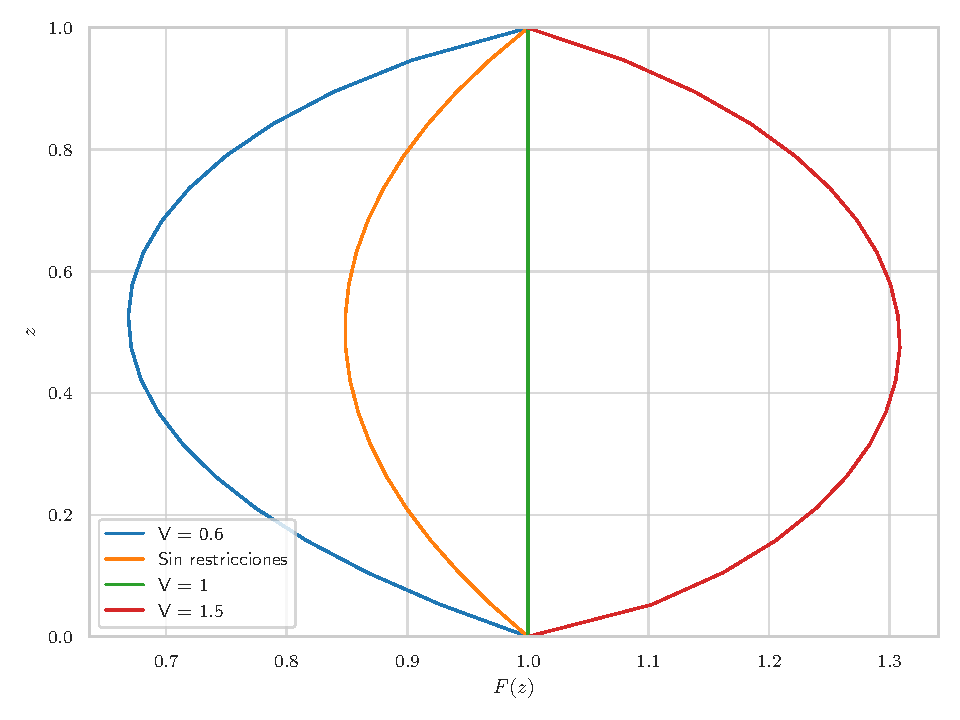
\includegraphics[width=\textwidth]{Figures/01/vol_inic_de.pdf}
        \caption{Soluciones válidas.}
        \label{fig:vol_inic_de}
    \end{subfigure}
    \hfill
    \begin{subfigure}[b]{0.45\textwidth}
        \centering
        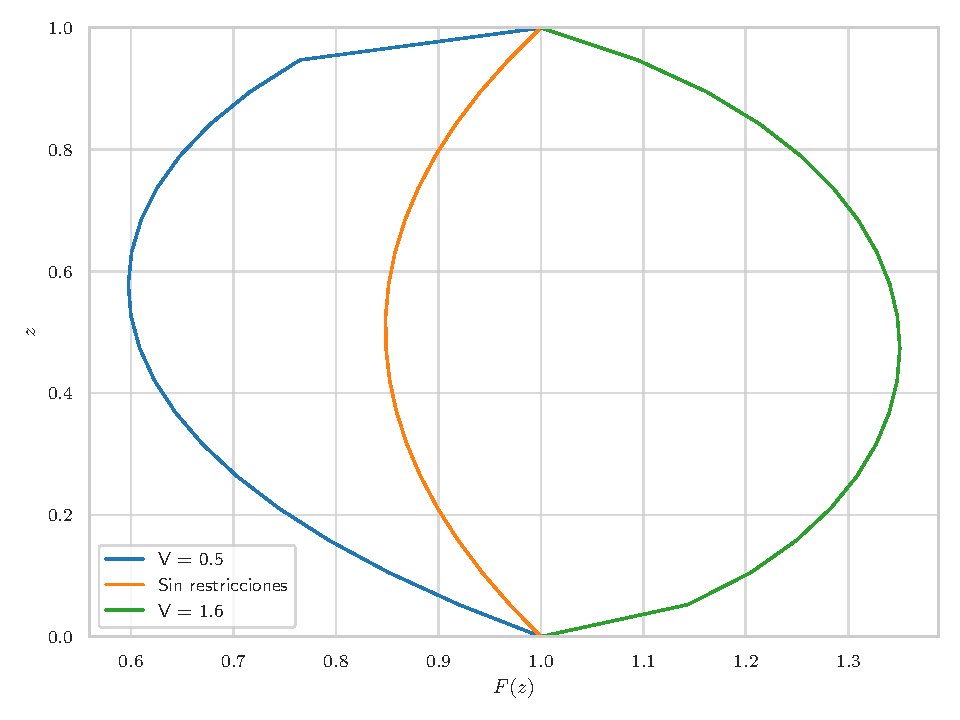
\includegraphics[width=\textwidth]{Figures/01/vol_no_sol_de.pdf}
        \caption{Soluciones no válidas.}
        \label{fig:vol_no_sol_de}
    \end{subfigure}
    \caption{Solución para distintos valores de la restricción de volumen, con método heurístico.}
    \label{fig:vol_variacion_de}
\end{figure}

Una vez más, las diferencias de tiempo son de varios órdenes de magnitud a favor del método gradiente, por lo que, como en el caso sin restricciones, se va a considerar la influencia de los parámetros modificándolos en el método gradiente únicamente, a fin de reducir el tiempo requerido para el análisis.

\subsection{Influencia de los parámetros en la solución}

En este apartado se van a comentar una pequeña parte de los parámetros analizados en \ref{ap:infl_params} sobre la solución para el método gradiente, ya que se ha estudiado la influencia de todos ellos y se ha concluido que no aportan información adicional a la recogida en dicho apartado. 

\subsubsection{Volumen fijado por la restricción}

Como se planteó en el apartado \ref{ap:cons_grad}, se va a modificar el número de puntos por si este pudiese influir en la precisión de las soluciones con valores cercanos a los límites donde la solución se calcula correctamente. En lugar de $n = 20$ tomado en cuenta para la primera aproximación, se va a emplear $n = 100$, por ser el valor más preciso según lo analizado en el apartado \ref{ap:infl_n}.

Como se puede apreciar en la Figura \ref{fig:vol_sol_n100}, al aumentar el número de puntos y, con ello, la precisión, se consigue obtener una solución para las restricciones de volumen de 0.5 y 1.6, así que queda patente que los resultados obtenidos en las Figuras \ref{fig:vol_variacion} y \ref{fig:vol_variacion_de} simplemente carecían de la precisión suficiente. 

\begin{figure}[h]
    \centering
    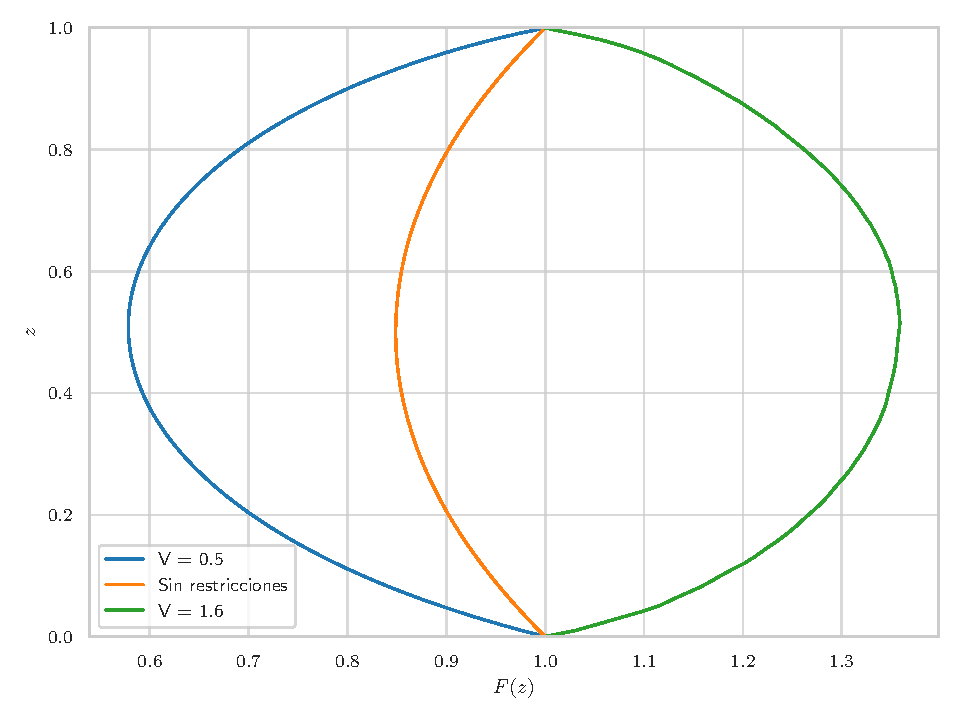
\includegraphics[width = 0.6 \linewidth]{Figures/01/vol_sol_n100.pdf}
    \caption{Solución para las restricciones que generaban complicaciones, con $n = 100$.}
    \label{fig:vol_sol_n100}
\end{figure}

Por tanto, surge la duda de dónde se encuentra el límite de la restricción para la que existe solución, por lo que, manteniendo $n = 100$, se va a buscar evaluar las restricciones para valores más lejanos del valor del volumen sin restricciones. En la Figura \ref{fig:vol_no_sol_n100} se aprecia que, para valores de V de 1.7 y 0.4, por mucho que se varíe el número de puntos, esto no da lugar a ninguna solución aceptable, por lo que se concluye que la restricción de volumen, para valores de $F_0 = 1$, ha de cumplir las siguientes condiciones:

\begin{equation}
    \boxed{0.4 < V < 1.7}
\end{equation}

\begin{figure}[h]
    \centering
    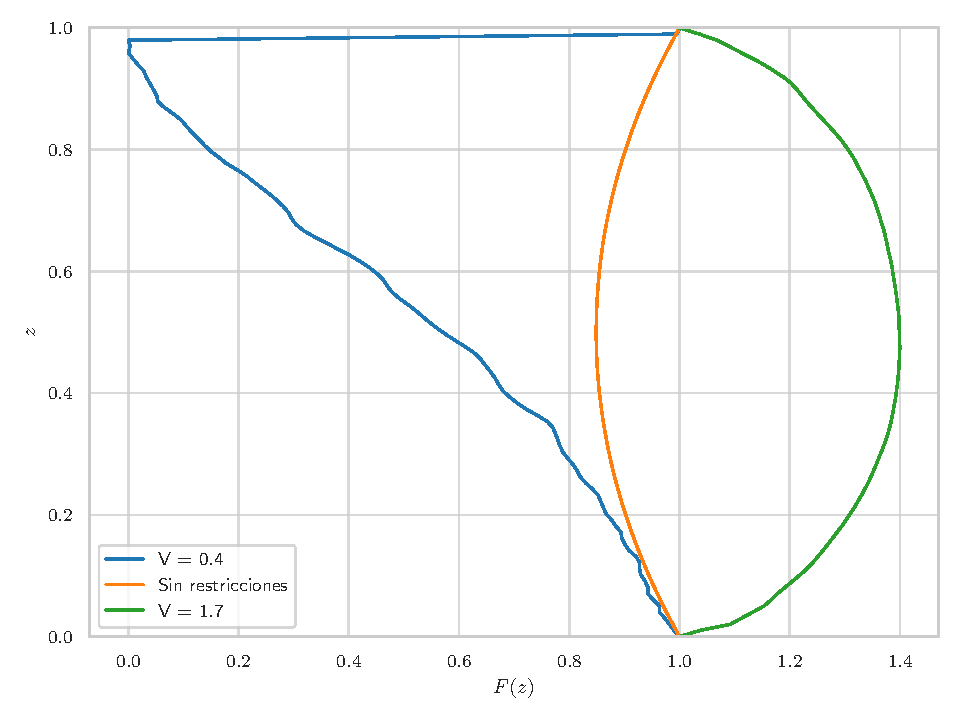
\includegraphics[width = 0.6 \linewidth]{Figures/01/vol_no_sol_n100.pdf}
    \caption{Solución para las restricciones que no tienen solución, con $n = 100$.}
    \label{fig:vol_no_sol_n100}
\end{figure}


\subsection{Influencia de la distribución de puntos}

Además de los efectos que tiene la distribución de puntos ya comentados en el apartado \ref{ap:infl_distrib}, en esta ocasión se va a comentar la influencia de la distribución de puntos en el caso muy particular de $V = 1$, el cual se puede relacionar muy fácilmente con la solución exacta al problema (un cilindro recto).

\begin{figure}[h]
    \centering
    \begin{subfigure}[b]{0.45\textwidth}
        \centering
        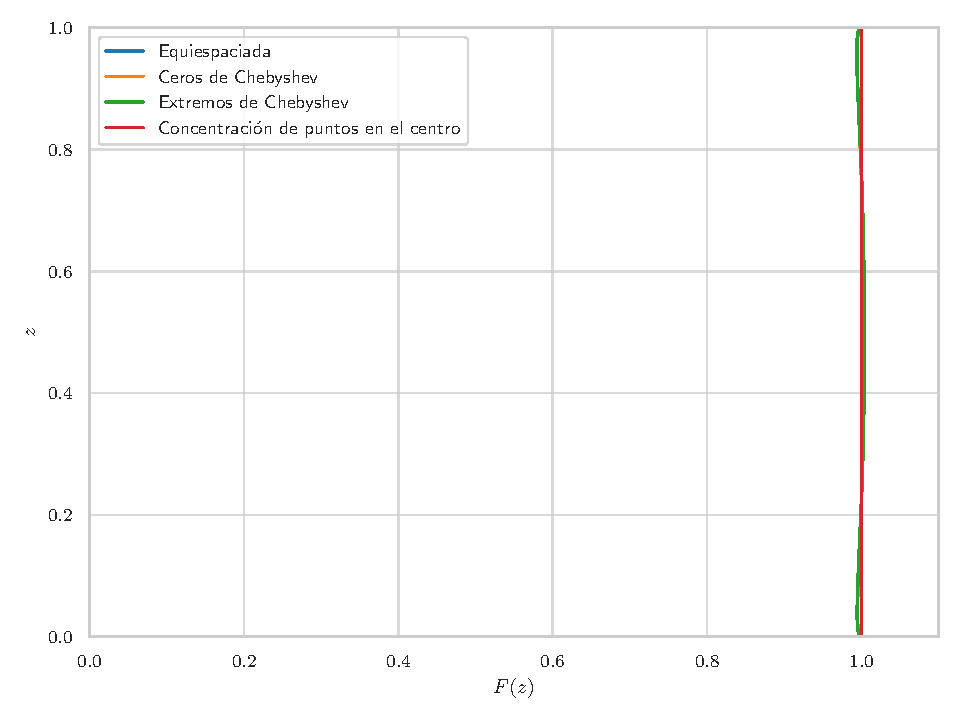
\includegraphics[width=\textwidth]{Figures/01/sol_vol1_lejos.pdf}
        \caption{}
        \label{fig:sol_vol1_lejos}
    \end{subfigure}
    \hfill
    \begin{subfigure}[b]{0.45\textwidth}
        \centering
        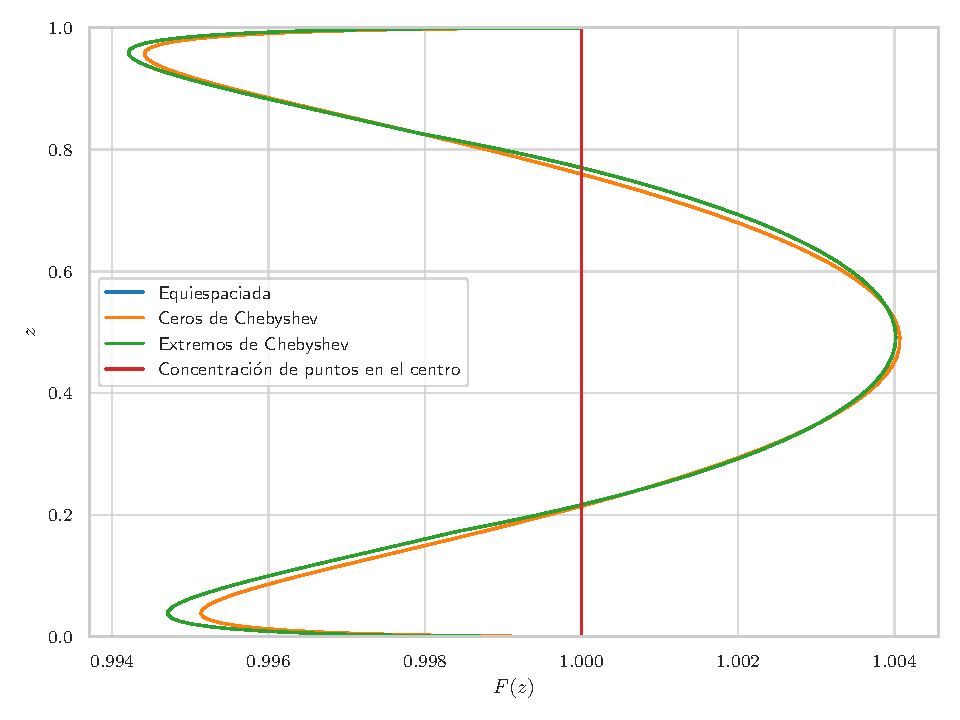
\includegraphics[width=\textwidth]{Figures/01/sol_vol1_cerca.pdf}
        \caption{}
        \label{fig:sol_vol1_cerca}
    \end{subfigure}
    \caption{Solución para $V = 1$.}
    \label{fig:sol_vol1}
\end{figure}

A primera vista, como se aprecia en la Figura \ref{fig:sol_vol1_lejos}, todas las soluciones son extremadamente similares, por lo que se pueden considerar todas igual de válidas. Sin embargo, al ampliar y observar la solución de una forma más cercana (Figura \ref{fig:sol_vol1_cerca}), se aprecia que la única que cumple la restricción de $V = 1$ y además se corresponde con la solución esperada es la equiespaciada. 

No se ha conseguido encontrar una explicación convincente a dicho fenómeno, pero, puesto que las escalas hacen que sea despreciable, se decide no darle más importancia.


\subsection{Consideraciones particulares}

\subsubsection{Restricción de volumen igual a la del problema libre}

En este apartado, se plantea el efecto que podría tener restringir el volumen al mismo que se obtiene de la solución sin restricciones. Los efectos que se quieren estudiar es si este cambio modifica el cálculo de la solución, es decir, si para llegar a la misma solución, por el hecho de imponer restricciones, requiere más tiempo o más iteraciones.

En contra de lo que pudiera parecer intuitivo, tanto en el método gradiente como en el heurístico, se ha podido comprobar que no aumenta el número de iteraciones requerido en ninguno de los dos casos, así como tampoco el tiempo de cálculo. De hecho, en las pruebas realizadas con el algoritmo DE, tanto el tiempo como las iteraciones se reducen, hecho que podría deberse precisamente a la imposición de la restricción, aunque también puede tratarse de una coincidencia fruto del azar que rige este método.


\section{Problema sin restricciones, con soportes de distinto tamaño}

A continuación, se considera el caso en el que ambos soportes no son iguales, por lo que las condiciones de contorno impuestas anteriormente se sustituyen por las siguientes:

\begin{equation} \label{eq:soportes}
    \begin{cases}
        F(0) = F_0 - \varepsilon \\
        F(1) = F_0 + \varepsilon
    \end{cases}
\end{equation}

Con esto, el problema pierde su simetría, por lo que se presume que aumentará la potencia de cálculo requerida para encontrar una solución, además de poder introducir otras complicaciones que se van a comentar a continuación. Sin embargo, una ventaja de considerar el problema sin restricciones es que otra vez se puede emplear la catenaria (ajustada correctamente) para calcular el error que presenta la solución.


\subsection{Minimización con método basado en gradiente}

En primer lugar, se considera la solución calculada mediante un método gradiente. No se va a incidir en ello, ya que la única diferencia con lo considerado en el apartado \ref{ap:params} es la variación del tamaño de los soportes, con un valor arbitrariamente pequeño de $\varepsilon = 0.1$, según la expresión \ref{eq:soportes}. Esta solución se representa en la Figura \ref{fig:sol_eps_SLSQP} y sus valores de error se comentarán más adelante.

\begin{figure}[h]
    \centering
    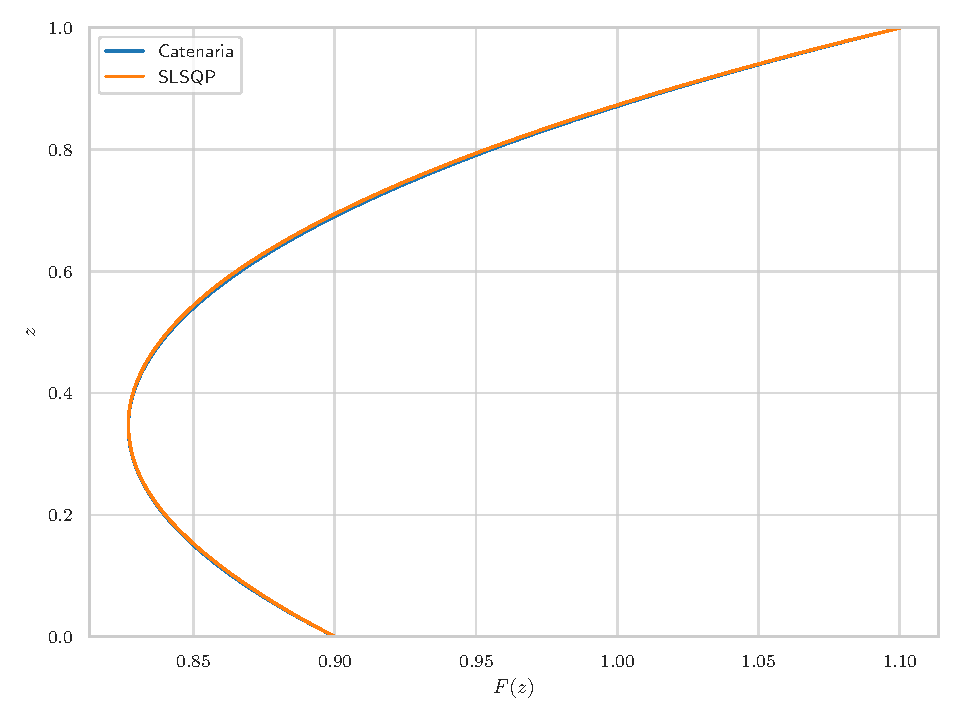
\includegraphics[width = 0.6 \linewidth]{Figures/01/sol_eps_SLSQP.pdf}
    \caption{Solución para $\varepsilon = 0.1$ con el método SLSQP.}
    \label{fig:sol_eps_SLSQP}
\end{figure}


\subsection{Minimización con un método heurístico}

Una vez más, en la Figura \ref{fig:sol_eps_de} se presenta la solución idéntica al caso anterior, en la que se representan tanto la solución obtenida por iteración con la parte evolutiva de \textit{Differential Evolution} como la solución del algoritmo híbrido que se ha implementado.

\begin{figure}[h]
    \centering
    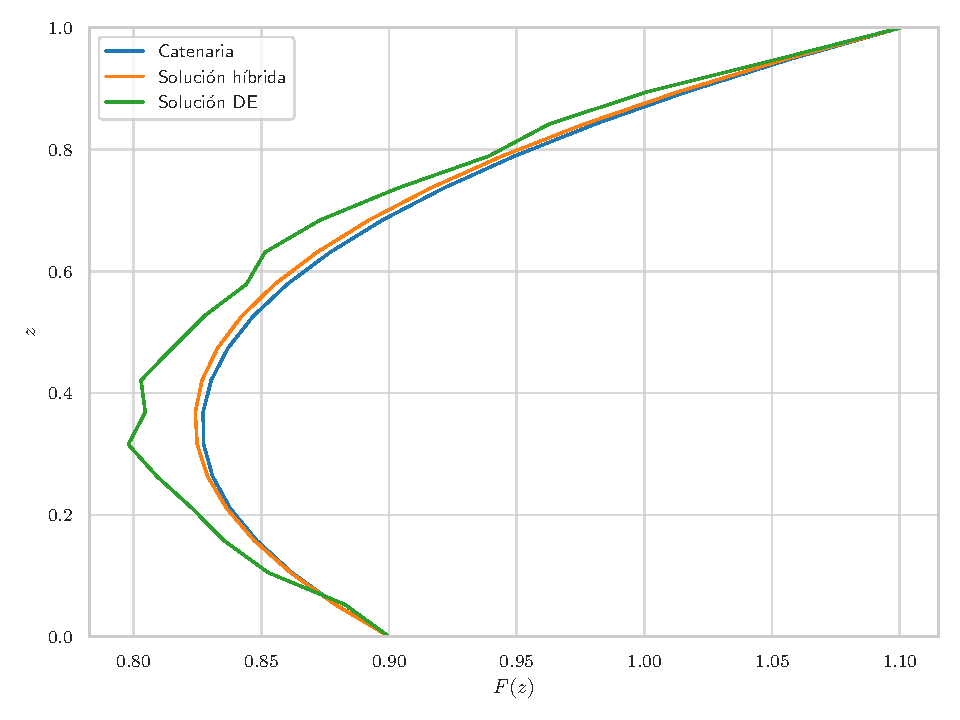
\includegraphics[width = 0.6 \linewidth]{Figures/01/sol_eps_de.pdf}
    \caption{Solución para $\varepsilon = 0.1$ con \textit{Differential Evolution}.}
    \label{fig:sol_eps_de}
\end{figure}

\subsection{Comparación entre el algoritmo tipo gradiente y el heurístico} 

Al igual que en el apartado \ref{ap:comp_alg}, se van a comparar los resultados obtenidos por ambos algoritmos a través de los valores de error obtenidos de calcular el error a partir de la catenaria.

\begin{table}[h]
    \centering
    \caption{Error para los algoritmos considerados, con soportes distintos.}
    \begin{tabular}{c c}
        \hline
        \textbf{Algoritmo} & \textbf{SLE} [\%] \\ \hline \hline   
        SLSQP & 0.370 \\ \hline
        DE (detención de la evolución) & 1.990 \\ \hline
        DE afinado con L-BFGS-B & 0.379 \\ \hline
    \end{tabular}
    \label{tab:error_algs_sop}
\end{table}

Como era de esperar, la Tabla \ref{tab:error_algs_sop} mantiene una tendencia similar a la mostrada en el apartado \ref{ap:comp_alg}: el algoritmo híbrido y el basado en gradiente son los que presentan menor valores del error, mientras que la solución obtenida exclusivamente mediante un algoritmo evolutivo es la más imprecisa. Como se mantienen las tendencias (también en tiempos de procesado), se recurre al algoritmo tipo gradiente para evaluar la influencia de los parámetros en la solución.


\subsection{Influencia de los parámetros en la solución}

Además de los parámetros ya estudiados en \ref{ap:infl_params} (que carecen de relevancia, puesto que la solución se comporta igual que en dicho caso), en este caso se presenta una nueva variable, $\varepsilon$, de la cual se va a estudiar su efecto en este apartado.

\subsubsection{Separación de los soportes, $\varepsilon$}

En realidad, analizando la ecuación \ref{eq:soportes}, la magnitud $\varepsilon$ representa la mitad de la diferencia entre los radios de ambos soportes. Es decir, si $\varepsilon = 0.1$, los valores de los soportes son $F(0) = 0.9$ y $F(1) = 1.1$.

A continuación, se va a evaluar para qué valores de $\varepsilon$ el problema tiene solución. En la Figura \ref{fig:sol_var_epsn20} se recoge la representación de la solución para diversos valores de $\varepsilon$, desde 0.0 a 0.4. Para el valor mayor, se observa que la solución calculada presenta errores grandes. 

\begin{figure}[h]
    \centering
    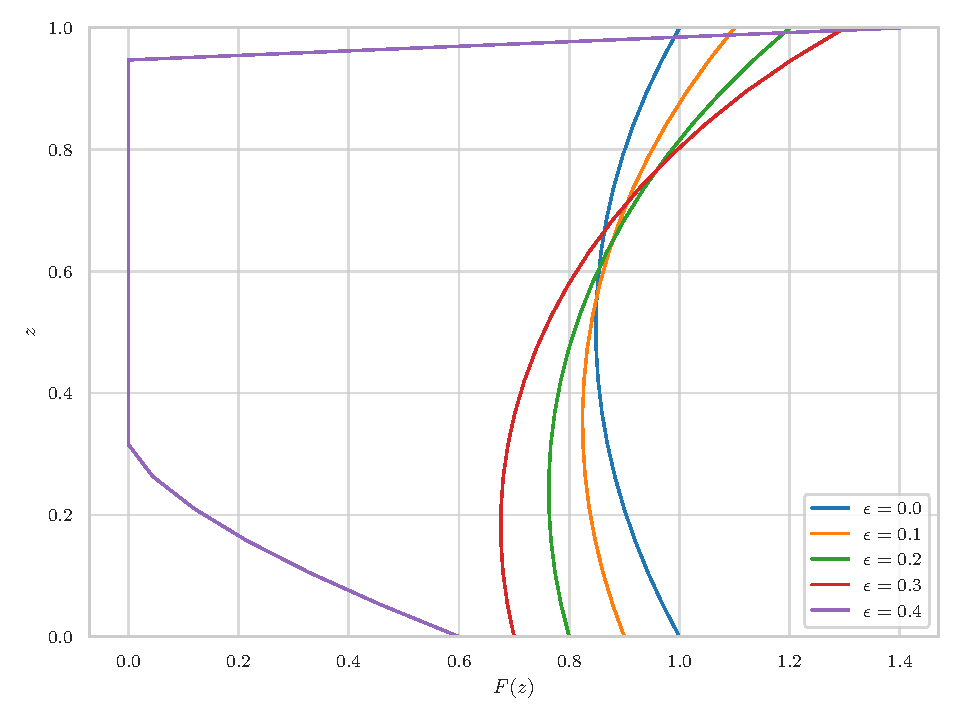
\includegraphics[width = 0.6 \linewidth]{Figures/01/sol_var_epsn20.pdf}
    \caption{Solución para el problema con soportes de diferente tamaño, con $n = 20$.}
    \label{fig:sol_var_epsn20}
\end{figure}

Esto puede ser debido, al igual que para el caso de las restricciones de volumen, a un error de precisión numérica por la división del intervalo. Al igual que en el resto del trabajo, se parte de una base de $n = 20$ con la que se calcularon los valores de la solución. A fin de mejorar la precisión de la solución y descubrir si esta existe o no, para el análisis que se llevará a cabo a continuación, se aumenta a $n = 100$, ya que esta es la que ha dado mejores resultados de precisión los estudios previos.

Así, en la Figura \ref{fig:sol_var_epsn100} se observa que, aumentando el número de puntos hasta $n = 100$, el problema admite solución hasta, por lo menos, $\varepsilon = 0.5$, por lo que el resultado obtenido en la Figura \ref{fig:sol_var_epsn20} se debía a fallos de precisión por considerar menos puntos de los necesarios para alcanzar la precisión suficiente. 

\begin{figure}[h]
    \centering
    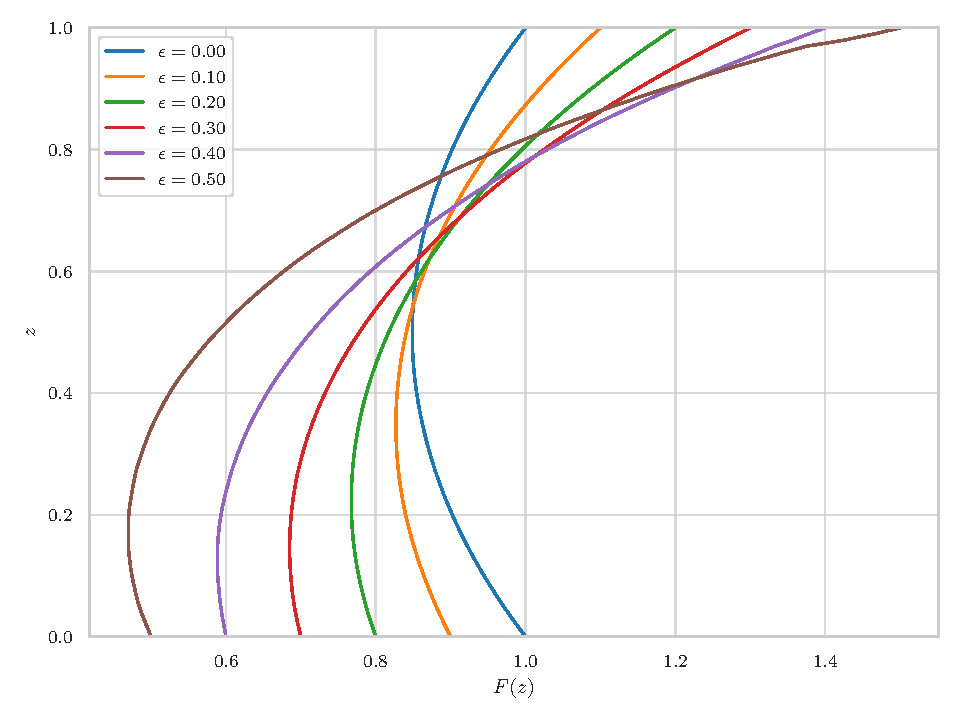
\includegraphics[width = 0.6 \linewidth]{Figures/01/sol_var_epsn100.pdf}
    \caption{Solución para el problema con soportes de diferente tamaño, con $n = 100$.}
    \label{fig:sol_var_epsn100}
\end{figure}

Considerando esto, se propone averiguar el valor máximo de $\varepsilon$ para el que el problema admite solución. Esto se realizará iterando sobre aumentos de $\varepsilon$ de 0.01 en cada paso, según se muestra en la Figura \ref{fig:sol_var_epsn100_cont}. 

\begin{figure}[!h]
    \centering
    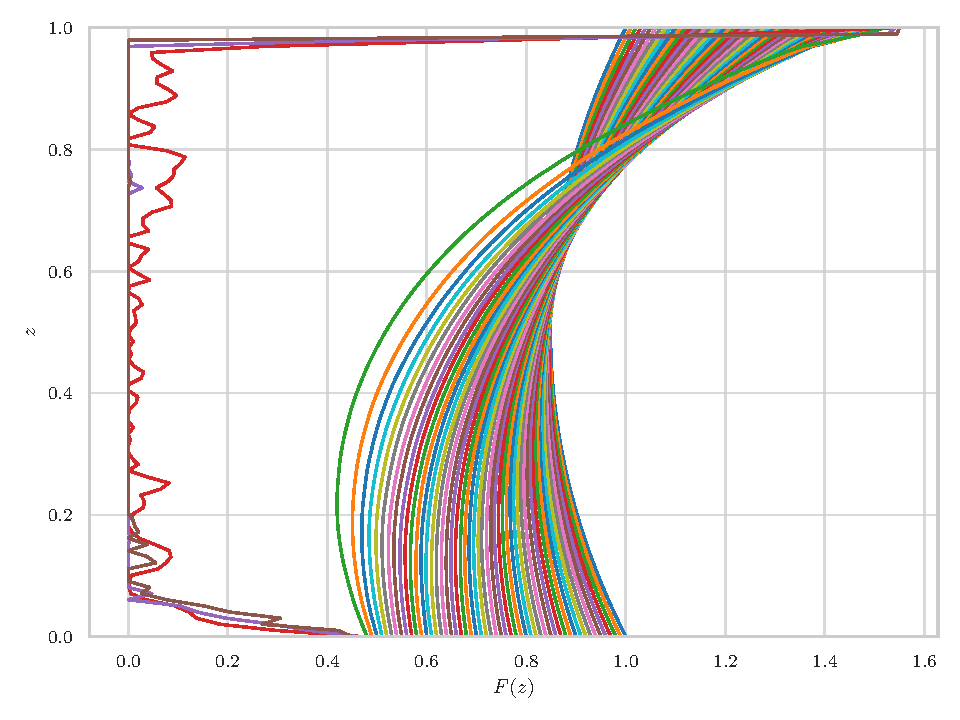
\includegraphics[width = 0.6 \linewidth]{Figures/01/sol_var_epsn100_cont.pdf}
    \caption{Solución para el problema con variaciones pequeñas del tamaño de los soportes.}
    \label{fig:sol_var_epsn100_cont}
\end{figure}

\begin{table}[h]
    \caption{Error para diferentes diferencias en los radios de los soportes, con $n = 100$.}
    \centering
    \begin{tabular}{c c}
        \hline
        $\varepsilon$ & \textbf{SLE [\%]} \\ \hline \hline
        0.00 &  0.039 \\ \hline
        0.10 &  0.116 \\ \hline
        0.20 &  0.273 \\ \hline
        0.30 &  0.397 \\ \hline
        0.40 &  1.083 \\ \hline
        0.50 &  4.955 \\ \hline
        0.51 &  6.383 \\ \hline
        0.52 &  9.680 \\ \hline
        0.53 & 89.439 \\ \hline
    \end{tabular}
    \label{tab:error_sop_n100}
\end{table}

De los valores de la Tabla \ref{tab:error_sop_n100} y de las representaciones de la Figura \ref{fig:sol_var_epsn100_cont} se aprecia que el valor de $\varepsilon$ límite es aproximadamente 0.53. Por debajo de este valor, el error crece con $\varepsilon$, pero se mantiene dentro de unos valores admisibles. Sin embargo, cuando $\varepsilon \geq 0.53$, el error supera valores para nada aceptables y, de las soluciones de la Figura \ref{fig:sol_var_epsn100_cont}, se observa que carecen de sentido y son debidas a que, realmente, no existe la solución para dichos valores de $\varepsilon$.


\section{Conclusión}

El análisis llevado a cabo en este trabajo ha permitido evaluar y comparar diferentes métodos de optimización, así como entender la influencia de la discretización y otros parámetros en la solución un problema de optimización real, con y sin restricciones y mediante la aplicación de diversos procesos estudiados en la asignatura. A continuación, se destacan los puntos clave de los hallazgos:

\begin{enumerate}
    \item \textbf{Métodos de Optimización}:
    \begin{itemize}
        \item \textbf{Método Basado en Gradiente}: Se ha observado que el método \textit{Sequential Least Squares Programming} (SLSQP) es efectivo y eficiente para resolver el problema que se presenta. Este método proporciona soluciones precisas con un bajo tiempo de cálculo, especialmente cuando el número de puntos de discretización es moderado.
        \item \textbf{Método Heurístico}: \textit{Differential Evolution} (DE) también se ha mostrado como una técnica robusta para la optimización global, siendo capaz de manejar bien el espacio de búsqueda multidimensional. Sin embargo, DE puede requerir un tiempo de cálculo significativamente mayor en comparación con los métodos basados en gradiente. El uso de una combinación híbrida de DE con un refinamiento posterior mediante un método de gradiente ha demostrado ser una estrategia eficaz para obtener soluciones precisas y razonablemente rápidas.
    \end{itemize}
    
    % \item \textbf{Distribución de Puntos}:
    % \begin{itemize}
    %     \item \textbf{Equiespaciada}: La distribución equiespaciada proporciona una solución general y equilibrada, aunque puede no capturar con precisión las variaciones rápidas en regiones con alta curvatura.
    %     \item \textbf{Ceros y Extremos de Chebyshev}: Estas distribuciones minimizan el error de interpolación y son particularmente útiles para evitar las oscilaciones de Runge. No obstante, se han observado oscilaciones inesperadas que pueden deberse a problemas de condicionamiento o a la falta de un manejo adecuado de las derivadas y restricciones en la optimización.
    %     \item \textbf{Concentración de Puntos en el Centro}: Esta distribución mejora la precisión en el centro del intervalo, capturando detalles finos en esa región, pero puede ser menos efectiva en los extremos.
    % \end{itemize}
    
    \item \textbf{Influencia de los Parámetros}:

    Como cualquier problema numérico, la elección de los parámetros que intervienen en el proceso es crucial en la solución de este. Una de las claves de una buena optimización, además de la obtención de la solución óptima del problema considerado, es hacer una gestión eficiente de los recursos disponibles. Es decir, puede ser más conveniente obtener una solución con unas tolerancias más relajadas si así se consigue reducir el tiempo de cálculo una cantidad importante. Por ello, la optimización de cualquier problema requiere llegar a un compromiso entre las variables que intervienen en este, tanto las intrínsecas como las extrínsecas a este. 
    % \begin{itemize}
    %     \item \textbf{Número de Puntos}: Un número moderado de puntos (por ejemplo, $n = 20$) proporciona un buen equilibrio entre precisión y tiempo de cálculo. Tanto un número demasiado bajo como demasiado alto de puntos puede introducir errores significativos debido a la falta de precisión o al error de redondeo.
    %     \item \textbf{Distribuciones no Equiespaciadas}: En casos con discretización alta, las distribuciones no equiespaciadas acumulan puntos de manera que reducen el error de redondeo y mejoran la adaptación a las características locales de la curva.
    %     \item \textbf{Valor de Arranque}: La elección del valor de arranque es crucial para la convergencia a la solución óptima. Valores de arranque incorrectos pueden llevar a soluciones no válidas, mientras que una adecuada proximidad a la solución esperada mejora la robustez del algoritmo.
    % \end{itemize}
\end{enumerate}

En resumen, el uso de métodos de optimización, la elección de la distribución de puntos y el ajuste adecuado de los parámetros juegan un papel fundamental en la precisión y eficiencia de la solución de problemas que se tratan en la asignatura. La combinación de métodos heurísticos con refinamiento basado en gradiente se ha mostrado prometedora para abordar los desafíos de estos problemas de optimización, pese a requerir mayor potencia que los de tipo gradiente. 

Por ello, se concluye que, siempre que se pueda validar que la solución es adecuada y que no se ha atascado en ningún mínimo local u otros problemas de convergencia que pueden sufrir estos algoritmos, conviene utilizar una optimización basada en gradiente, como la SLSQP considerada en este trabajo, ya que sigue siendo más rápido y requiere menos esfuerzo de cálculo realizar unas pocas pruebas con este método que el tiempo que tarda un método heurístico en converger.


\nocite{numpy}
\clearpage


%   ---   BIBLIOGRAFÍA/REFERENCIAS   ---   %

\phantomsection
\addcontentsline{toc}{section}{Referencias}
\renewcommand{\refname}{Referencias}
% \bibliographystyle{elsarticle-num}
\bibliographystyle{plain} % Establecer el estilo de bibliografía
\bibliography{references.bib}
\clearpage



%   ---   ANEXOS   ---   %

% \appendix
% \renewcommand{\appendixname}{Anexos}
% \addcontentsline{toc}{section}{\appendixname}
% \clearpage % or \cleardoublepage
% \appendixpage
% \addappheadtotoc
% \renewcommand{\appendixname}{Anexo}


% \section{Título del anexo} \label{ap:montaje}

Aquí puedes meter la información que no sea imprescindible en el cuerpo del trabajo pero si que interese que esté en el documento.
% \clearpage



\end{document}